\documentclass{haxe}

% todo-related
\usepackage[left=4.7cm, right=2cm, top=2cm, bottom=4.2cm]{geometry}
\usepackage[draft]{todonotes}
\reversemarginpar

% title (TODO: move this to class file once it looks good)

\renewcommand{\maketitle}{
   \begin{titlepage}
     \setcounter{page}{-1}
			\begin{center}
				~\\[3cm]
				
\includegraphics[scale=1.25]{assets/logo.pdf}~\\[1cm]
				{\huge \bfseries Haxe 3 Manual}\\[7cm]
				Haxe Foundation\\
				\today
			\end{center}
   \end{titlepage}
}




\begin{document}
\title{Haxe 3 Manual}
\author{Haxe Foundation}
\date{\today}
\maketitle


\clearpage
\todototoc
\listoftodos
\clearpage

\clearpage
\tableofcontents
\clearpage

\chapter{Introduction}
\label{introduction}
\state{NoContent}

\section{What is Haxe?}
\label{introduction-what-is-haxe}

Haxe is a high-level, open source programming language and compiler. It allows compilation of programs written using an ECMAScript\footnote{http://www.ecma-international.org/publications/standards/Ecma-327.htm}-oriented syntax to multiple target languages. Employing proper abstraction, it is possible to maintain a single code-base which compiles to multiple targets.

Haxe is strongly typed, but the typing system can be subverted where required. Utilizing type information, the Haxe type system can detect errors at compile-time which would only be noticeable at runtime in the target language. Furthermore, type information can be used by the target generators to generate optimized and robust code.

Currently, there are eight supported target languages which allow different use-cases:

\begin{center}
\begin{tabular}{| l | l | l |}
	\hline
	Name & Output type & Main usages \\ \hline
	Javascript & Sourcecode & Desktop, Mobile, Server \\
	Actionscript 3 & Sourcecode & Browser, Desktop, Mobile \\
	Flash & Bytecode & Browser, Desktop, Mobile \\ 
	Neko & Bytecode & Desktop, Server \\
	PHP & Sourcecode & Server \\
	C++ & Sourcecode & Desktop, Mobile, Server \\
	Java & Sourcecode & Desktop, Server \\
	C\# & Sourcecode & Desktop, Mobile, Server \\ \hline
\end{tabular}
\end{center}
The remainder of section \ref{introduction} gives a brief overview of what a Haxe program looks like, and how Haxe evolved since its inception in 2005.

\Fullref{types} introduces the seven different kinds of types in Haxe and how they interact with each other. The discussion of types is continued in \Fullref{type-system}, where features like \emph{unification}, \emph{type parameters} and \emph{type inference} are explained.

\Fullref{class-field} is all about the structure of Haxe classes and, among other topics, deals with \emph{properties}, \emph{inline fields} and \emph{generic functions}.

In \Fullref{expression} we see how to actually get programs to do something by using \emph{expressions}, plenty of which are used in the Haxe Standard Library described in \Fullref{std}.

\Fullref{lf} describes some of the Haxe features in detail, such as \emph{pattern matching}, \emph{string interpolation} and \emph{dead code elimination}.

Finally, we will venture to the exciting land of \emph{haxe macros} in \Fullref{macro} to see how some common tasks can be greatly simplified.


\section{About this Document}
\label{introduction-about-this-document}

This document is the official manual for Haxe 3. As such, it is not a beginner's tutorial and does not teach programming. However, the topics are roughly designed to be read in order and there are references to topics ``previously seen'' and topics ``yet to come''. In some cases, an earlier section makes use of the information of a later section if it simplifies the explanation. These references are linked accordingly and it should generally not be a problem to read ahead on other topics.

We use a lot of Haxe source code to keep a practical connection of theoretical matters. These code examples are often complete programs that come with a main function and can be compiled as-is. However, sometimes only the most important parts are shown.
Source code looks like this:

\begin{lstlisting}
Haxe code here
\end{lstlisting}
Occasionally, we demonstrate how Haxe code is generated, for which we usually show the \target{Javascript} target.

Furthermore, we define a set of terms in this document. Most often, this is done when introducing a new type or when a term is specific to Haxe. We not define every new aspect we introduce, e.g. what a class is, in order to not clutter the text. A definition looks like this:
\define{Definition name}{Definition description}

In a few places, this document has \emph{trivia}-boxes. These include off-the-record information such as why certain decisions were made during Haxe's development or how a particular feature has been changed in past Haxe versions. This information is generally not important and can be skipped as it is only meant to convey trivia:

\trivia{About Trivia}{This is trivia.}

\subsection{Authors and contributions}
\label{introduction-authors-and-contributions}

Most of this document's content was written by Simon Krajewski while working for the Haxe Foundation. We would like to thank these people for their contributions:

\begin{itemize}
	\item Dan Korostelev: Additional content and editing
	\item Caleb Harper: Additional content and editing
	\item Josefiene Pertosa: Editing
	\item Miha Lunar: Editing
\end{itemize}



\section{Hello World}
\label{introduction-hello-world}

The following program prints ``Hello World'' after having been compiled and run:

\haxe{assets/HelloWorld.hx}
This can be tested by saving the above code to a file named \ic{HelloWorld.hx} and invoking the Haxe Compiler like so: \ic{haxe -main HelloWorld --interp}. This generates the following output: \ic{HelloWorld.hx:3: Hello world}. There are several things to learn from this:

\begin{itemize}
	\item Haxe programs are saved in files with an extension of \ic{.hx}.
	\item The Haxe Compiler is a command-line tool which can be invoked with parameters such as \ic{-main HelloWorld} and \ic{--interp}.
	\item Haxe programs have classes (\type{HelloWorld}, upper-case), which have functions (\expr{main}, lower-case). 
\end{itemize}

\section{History}
\label{introduction-haxe-history}
\state{Edited}

The Haxe project started on 22 October 2005 as a successor to the \emph{Motion-Twin Action Script Compiler}, MTASC. French developer \emph{Motion-Twin}\footnote{http://motion-twin.org} had developed MTASC as a popular ActionScript 2 compiler, and the next logical step for them was to design their very own programming language; thus, giving birth to Haxe.

Being spelled \emph{haXe} back then, its beta was released in February 2006 with the first supported targets being AVM\footnote{Adobe Virtual Machine}-bytecode and Motion-Twin's own \emph{Neko} virtual machine\footnote{http://nekovm.org}.

\emph{Nicolas Cannasse}, who remains leader of the Haxe project to this date, kept on designing Haxe with a clear vision, subsequently leading to the Haxe 1.0 release in May 2006. This first major release came with support for \target{Javascript} code generation and already had some of the features that define Haxe today, such as type inference and structural sub-typing.

Haxe 1 saw several minor releases over the course of two years, adding the \target{Flash 9} target along with the \emph{haxelib}-tool in August 2006 and the \target{Actionscript 3} target in March 2007. During these months, there was a strong focus on improving stability, which came in the form of several minor bug-fix releases.

Haxe 2.0 was released in July 2008, coming with the \target{PHP} target courtesy of \emph{Franco Ponticelli}. A similar effort by \emph{Hugh Sanderson} lead to the addition of the \target{C++} target in July 2009 with the Haxe 2.04 release.

Just as with Haxe 1, what followed were several months of stability releases. In January 2011, Haxe 2.07 was released with the support of \emph{macros}. Around that time, \emph{Bruno Garcia} joined the team as maintainer of the \target{Javascript} target, which saw vast improvements in the subsequent 2.08 and 2.09 releases.

After the release of 2.09, \emph{Simon Krajewski} joined the team and work towards Haxe 3 began. Furthermore, \emph{Cau\^{e} Waneck}'s \target{Java} and \target{C\#} targets found their way into the Haxe builds. It was then decided to make one final Haxe 2 release, which happened in July 2012 with the release of Haxe 2.10.

In late 2012, the Haxe 3 switch was flipped and the Haxe Compiler team, now backed by the newly established \emph{Haxe Foundation}\footnote{http://haxe-foundation.org}, focused on this next major version. Haxe 3 was subsequently released in May 2013.

\part{Language Reference}

\chapter{Types}
\label{types}

The Haxe Compiler employs a sophisticated typing system which helps detecting type-related errors in a program at compile-time. A type error is an invalid operation on a given type, such as dividing by a String, trying to access a field of an Integer or calling a function with not enough (or too many) arguments.

In some languages this additional safety comes at a price because programmers are forced to explicitly assign types to syntactic constructs:

\begin{lstlisting}
var myButton:MySpecialButton = new MySpecialButton(); // As3
MySpecialButton* myButton = new MySpecialButton(); // C++ 
\end{lstlisting}
The explicit type annotations are not required in Haxe, because the compiler can \emph{infer} the type:

\begin{lstlisting}
var myButton = new MySpecialButton(); // Haxe
\end{lstlisting}
We will explore type inference in detail later in \Fullref{type-system-type-inference}. For now, it is sufficient to say that the variable \expr{myButton} in the above code is known to be an \emph{instance of class} \type{MySpecialButton}. A class instance is one of seven type groups:

\begin{description}
 \item[Class instance:] an object of a given class or interface
\todo{A class instance can be a class instance or something else? Somewhat confusing.}
 \item[Enum instance:] a value of a Haxe enumeration
 \item[Structure:] an anonymous structure, i.e. a collection of named fields
 \item[Function:] a compound type of several arguments and one return
 \item[Dynamic:] a wildcard type which is compatible to any type
 \item[Abstract:] an abstract value type
\todo{``abstract value type'' doesn't really provide any explanation}
 \item[Monomorph:] an unknown type, which may later become a different type
\end{description}

\define{Compound Type}{A compound type is a type which has sub-types. This includes any type with \tref{type parameters}{type-system-type-parameters} and the \tref{function}{types-function} type.}


\section{Basic Types}
\label{types-basic-types}

\todo{Check wording here (we don't want to address ``you'')}

\todo{A bit heavy on jargon. I don't know what abstract types are, what :coreType means, what metadata refers to and all the other stuff, but the section references and warnings are good to have.}

\emph{Basic Types} include \emph{Bool, Float, and Int}.  The basic types are \emph{abstract types} tagged with \emph{:coreType} metadata.  This means is they get replaced by platform specific types at compile-time.  Don't worry about all of the implementation details at the moment, but feel free to see \Fullref{types-abstract} and \Fullref{lf-metadata} for more details.  Just be aware that this abstraction can cause the \Fullref{types-overflow} and \Fullref{types-nullability} of Basic Types to behave differently on different target platforms.  To reiterate: \textbf{basic types can behave differently depending on the target platform.}

\subsection{Numeric types}
\label{types-numeric-types}

\define[Type]{Float}{Represents a double-precision IEEE 64-bit floating point number.}
\define[Type]{Int}{Represents an integral number.}
While every \type{Int} can be used where a \type{Float} is expected (that is, \type{Int} \emph{is assignable to} or \emph{unifies with} \type{Float}), the reverse is not true: Assigning a \type{Float} to an \type{Int} might lose precision and is not implicitly allowed.

\subsection{Overflow}
\label{types-overflow}

\todo{Took the ideas from old manual, but moved Neko in with C++ and co.  Still Haxe 3 relevant?}For performance reasons, the Haxe Compiler does not enforce any overflow behavior.  The burden of checking for overflows falls to the target platform. Here are some platform specific notes on overflow behavior:

\todo{Markdown: prettier formatting (bold definition names)}

\begin{description}
 \item[C++, Java, C\#, Neko:] 32-bit integers, with usual overflow practices. 
 \item[Flash, AVM2:] 32-bit integers, but higher integers are memory boxed.
 \todo{``Flash, AVM2'' looks like two different things, perhaps Flash 9+ (AVM2) is clearer? How high? Memory boxed? What is this and what are the implications?}
 \item[PHP, JS, Flash 8:] No native \emph{Int} type.  Overflows will occur if they reach their float limit (2\textsuperscript{52}).
\end{description}

Alternatively, the \emph{haxe.Int32} and \emph{haxe.Int64} classes can be used to ensure correct overflow behavior regardless of the platform.  

\subsection{Numeric Operators}
\label{types-numeric-operators}

\todo{make sure the types are right for inc, dec, negate, and bitwise negate}
\begin{center}
\begin{tabular}{| l | l | l | l | l |}
	\hline
	\multicolumn{5}{|c|}{Arithmetic} \\ \hline
	Operator & Operation & Argument 1 & Argument 2 & Return \\ \hline
	\expr{++}& increment & \type{Int} & \type{N/A} & \type{Int}\\
	& & \type{Float} & \type{N/A} & \type{Float}\\
	\expr{--} & decrement & \type{Int} & \type{N/A} & \type{Int}\\
	& & \type{Float} & \type{N/A} & \type{Float}\\
	\expr{+} & addition & \type{Float} & \type{Float} & \type{Float} \\
	& & \type{Float} & \type{Int} & \type{Float} \\
	& & \type{Int} & \type{Float} & \type{Float} \\
	& & \type{Int} & \type{Int} & \type{Int} \\
	\expr{-} & subtraction & \type{Float} & \type{Float} & \type{Float} \\
	& & \type{Float} & \type{Int} & \type{Float} \\
	& & \type{Int} & \type{Float} & \type{Float} \\
	& & \type{Int} & \type{Int} & \type{Int} \\
	\expr{*} & multiplication & \type{Float} & \type{Float} & \type{Float} \\
	& & \type{Float} & \type{Int} & \type{Float} \\
	& & \type{Int} & \type{Float} & \type{Float} \\
	& & \type{Int} & \type{Int} & \type{Int} \\	
	\expr{/} & division & \type{Float} & \type{Float} & \type{Float} \\
	& & \type{Float} & \type{Int} & \type{Float} \\
	& & \type{Int} & \type{Float} & \type{Float} \\
	& & \type{Int} & \type{Int} & \type{Float} \\
	\expr{\%} & modulo & \type{Float} & \type{Float} & \type{Float} \\
	& & \type{Float} & \type{Int} & \type{Float} \\
	& & \type{Int} & \type{Float} & \type{Float} \\
	& & \type{Int} & \type{Int} & \type{Int} \\	 \hline
	\multicolumn{5}{|c|}{Comparison} \\ \hline
	Operator & Operation & Argument 1 & Argument 2 & Return \\ \hline
	\expr{\textasciitilde} & negation & \type{Float/Int} & \type{N/A} & \type{Bool} \\
	\expr{==} & equal & \type{Float/Int} & \type{Float/Int} & \type{Bool} \\
	\expr{!=} & not equal & \type{Float/Int} & \type{Float/Int} & \type{Bool} \\
	\expr{<} & less than & \type{Float/Int} & \type{Float/Int} & \type{Bool} \\
	\expr{<=} & less than or equal & \type{Float/Int} & \type{Float/Int} & \type{Bool} \\
	\expr{>} & greater than & \type{Float/Int} & \type{Float/Int} & \type{Bool} \\
	\expr{>=} & great than or equal & \type{Float/Int} & \type{Float/Int} & \type{Bool} \\ \hline
	\multicolumn{5}{|c|}{Bitwise} \\ \hline
	Operator & Operation & Argument 1 & Argument 2 & Return \\ \hline
	\expr{!} & bitwise negation & \type{Int} & \type{N/A} & \type{Int} \\	
	\expr{\&} & bitwise and & \type{Int} & \type{Int} & \type{Int} \\	
	\expr{|} & bitwise or & \type{Int} & \type{Int} & \type{Int} \\	
	\expr{\^} & bitwise xor & \type{Int} & \type{Int} & \type{Int} \\	
	\expr{<<} & shift left & \type{Int} & \type{Int} & \type{Int} \\
	\expr{>>} & shift right & \type{Int} & \type{Int} & \type{Int} \\
	\expr{>>>} & unsigned shift right & \type{Int} & \type{Int} & \type{Int} \\ \hline
\end{tabular}
\end{center}

\subsection{Bool}
\label{types-bool}

\define[Type]{Bool}{Represents a value which can be either \emph{true} or \emph{false}.}
Values of type \type{Bool} appear commonly in \emph{conditions} such as \expr{if} (section \ref{expression-if}) and \expr{while} (section \ref{expression-while}). The following \emph{operators} accept and return \type{Bool} values:
\begin{itemize}
	\item \expr{\&\&} (and)
	\item \expr{||} (or)
	\item \expr{!} (not)
\end{itemize}
Haxe guarantees that compound boolean expressions are evaluated from left to right and only as far as necessary at runtime. For instance, an expression like \expr{A \&\& B} will evaluate \expr{A} first and evaluate \expr{B} only if the evaluation of \expr{A} yielded \expr{true}. Likewise, the expressions \expr{A || B} will not evaluate \expr{B} if the evaluation of \expr{A} yielded \expr{true}, because the value of \expr{B} is irrelevant in that case.
This is important in some cases such as this:

\begin{lstlisting}
if (object != null && object.field == 1) { ... }
\end{lstlisting}
Accessing \expr{object.field} if \expr{object} is \expr{null} would lead to a runtime error, but the check for \expr{object != null} guards against it.




\subsection{Void}
\label{types-void}

\define[Type]{Void}{Void denotes the absence of a type. It is used to express that something (usually a function) has no value.}

\type{Void} is a special case in the type system because it is not actually a type. It is used to express the absence of a type, which applies mostly to function arguments and return types.
We have already ``seen'' Void in the initial ``Hello World'' example:

\haxe{assets/HelloWorld.hx}
The function type will be explored in detail in section \Fullref{types-function}, but a quick preview helps here: The type of function \expr{main} in above example can be considered to be \type{Void->Void}, which reads as ``it has no arguments and returns nothing''.
Haxe does not allow fields and variables of type \type{Void}, and will complain if an attempt is made at declaring such:

\begin{lstlisting}
var x:Void; // Arguments and variables of type Void are not allowed
\end{lstlisting}
\todo{Consider having special ``compiler error'' formatting, so it's fancier than a comment.}



\section{Nullability}
\label{types-nullability}

\define{nullable}{A type in Haxe is considered \emph{nullable} if \expr{null} is a valid value for it.}

It is common for programming languages to have a single, clean definition for nullability. However, Haxe has to find a compromise in this regard. The reason for this is obvious when looking at the nature of Haxe's target languages: While some of them allow and, in fact, default to \expr{null} for anything, others do not even allow \expr{null} for certain types. This necessitates the distinction of two types of target languages:

\define{Static target}{Static targets employ their own type system where \expr{null} is not a valid value for basic types. This is true for the \target{Flash 9+}, \target{C++}, \target{Java} and \target{C\#} targets.}
\define{Dynamic target}{Dynamic targets are more lenient with their types and allow \expr{null} values for basic types. They consist of \target{JavaScript}, \target{PHP}, \target{neko} and \target{Flash 6-8}.}

There is nothing to worry about when working with \expr{null} on dynamic targets, but static ones may require some thought. For starters, basic types are initialized to these values:

\begin{description}
	\item[\type{Int}:] \expr{0}
	\item[\type{Float}:] \expr{NaN} on \target{Flash 9+}, \expr{0.0} on other static targets
	\item[\type{Bool}:] \expr{false}
\end{description}
As a consequence, the Haxe Compiler does not allow the assignment of \expr{null} to a basic type on static targets. In order to achieve this, the basic type has to be wrapped as \type{Null$<$T$>$}:
\todo{\type{Null$<$T$>$} hasn't been mentioned before I think, so it could be confusing as to what it is and why it's there and how it works and why it works.}

\begin{lstlisting}
var a:Int = null; // error on static platforms
var b:Null<Int> = null; // allowed
\end{lstlisting}
Similarly, basic types cannot be compared to \expr{null} unless wrapped:

\begin{lstlisting}
var a : Int = 0;
if( a == null ) { ... } // error on static platforms
var b : Null<Int> = 0;
if( b != null ) { ... } // allowed
\end{lstlisting}
This restriction extends to all situations where \tref{unification}{type-system-unification} is performed.

If a \expr{null}-value is ``hidden'' in \type{Null$<$T$>$} or \type{Dynamic} and assigned to a basic type, the default value is used:

\begin{lstlisting}
var n : Null<Int> = null;
var a : Int = n;
trace(a); // 0 on static platforms
\end{lstlisting}

\emph{Optional Arguments and Nullability:}
\todo{This could be expanded upon and might be better as a subsection.}
Optional arguments also have to be accounted when considering nullability.
In particular, there must be a distinction between \emph{native} optional arguments which are not nullable and Haxe optional arguments which might be.  The distinction is made by using the question-mark optional argument:

\trivia{Argument vs Parameter}{In some other programming languages, \emph{argument} and \emph{parameter} are used interchangably.  In Haxe, \emph{argument} is used when referring to methods, and \emph{parameter} refers to \Fullref{type-system-type-parameters}.}
\todo{Trivia should probably be after example (but perhaps in a floating box that decides to position itself at the ends of pages or something, if that was the goal).}

\begin{lstlisting}
// x is a native Int (not nullable)
function foo(x : Int = 0) {...}
// y is Null<Int> (nullable)
function bar( ?y : Int) {...}
// z is also Null<Int>
function opt( ?z : Int = -1) {...}
\end{lstlisting}
\todo{Is there a difference between \type{?y : Int} and \type{y : Null$<$Int$>$} or can you even do the latter? Some more explanation and examples with native optional and Haxe optional arguments and how they relate to nullability would be nice.}



\section{Class Instance}
\label{types-class-instance}

Similar to many object-oriented languages, classes in Haxe are the primary data structure for the majority of programs. Each Haxe class has an explicit name, an implied path and zero or more class fields. Here we will focus on the general structure of classes and their relations, while leaving the details of class fields for \Fullref{class-field}.

The following code example serves as basis for the remainder of this section:

\haxe{assets/Point.hx}
\todo{Doesn't toString need return type of String?}
Semantically, this class represents a point in discrete 2-dimensional space, but this is not important here. Let us instead describe the structure:

\begin{itemize}
	\item The keyword \expr{class} denotes that we are declaring a class.
	\item \type{Point} is the name of the class and could be anything conforming to the \tref{rules for type identifiers}{expression-rules}.
	\item Enclosed in curly braces \expr{$\left\{\right\}$} are the class fields,
	\item which consist of two \emph{variable} fields \expr{x} and \expr{y} of type \type{Int},
	\item followed by a special \emph{function} field named \expr{new}, which is the \emph{constructor} of the class,
	\item as well as a normal function \expr{toString}.
\end{itemize}
There is a special type in Haxe which is compatible with all classes:

\define[Type]{Class$<$T$>$}{This type is compatible with all class types. At compile-time, \type{Class<T>} can be considered to be the common base type of all class types. However, this relation is not reflected in generated code.}
\todo{Same as in 2.2, what the \type{Class$<$T$>$} syntax means is unclear at this point.}
\todo{What are class types?}

\subsection{Class constructor}
\label{types-class-constructor}

Instances of classes are created by calling the class constructor, a process commonly referred to as \emph{instantiation}. Another name for class instances is \emph{object}, but we prefer the term class instance to emphasize the analogy between classes/class instances and \tref{enums/enum instances}{types-enum-instance}. 
\todo{Minor semantics: instances are created by calling the constructor or is the constructor called when they are created?}

\begin{lstlisting}
var p = new Point(-1, 65);
\end{lstlisting}
This will yield an instance of class \type{Point}, which is assigned to a variable named \expr{p}. The constructor of \type{Point} receives the two arguments \expr{-1} and \expr{65} and assigns them to the instance variables \expr{x} and \expr{y} respectively (compare its definition in \Fullref{types-class-instance}). We will revisit the exact meaning of the \expr{new} expression later in section \ref{expression-new}. For now, we just consider it as calling the class constructor and returning the appropriate object.



\subsection{Inheritance}
\label{types-class-inheritance}

Classes may inherit from other classes, which in Haxe is denoted by the \expr{extends} keyword:

\haxe{assets/Point3.hx}
This relation is often described as "is-a": Any instance of class \type{Point3} is also an instance of \type{Point}. \type{Point} is then known as the \emph{parent class} of \type{Point3}, which is a \emph{child class} of \type{Point}. A class may have many child classes, but only one parent class. The term ``a parent class of class X'' usually refers to its direct parent class, the parent class of its parent class and so on.

The code above is very similar to the original \type{Point} class, with two new constructs being shown:
\begin{itemize}
 \item \expr{extends Point} denotes that this class inherits from class \type{Point}
 \item \expr{super(x, y)} is the call to the constructor of the parent class, in this case \expr{Point.new}
\end{itemize}
It is not necessary for child classes to define their own constructors, but if they do, a call to \expr{super()} is mandatory. Unlike some other object-oriented languages, this call can appear anywhere in the constructor code and does not have to be the first expression.
\todo{Mandatory even if there are no arguments? (could be useful to mention as it's not in something like AS3 afaik)}

A class may override \tref{methods}{class-field-method} of its parent class, which requires the explicit \expr{override} keyword. The effects and restrictions of this are detailed in \Fullref{class-field-overriding}.


\subsection{Interfaces}
\label{types-interfaces}

An interface can be understood as the signature of a class because it describes the public fields of a class. Interfaces do not provide implementations, but rather pure structural information:

\begin{lstlisting}
interface Printable {
	public function toString():String;
}
\end{lstlisting}
The syntax is similar to classes, with the following exceptions:

\begin{itemize}
	\item \expr{interface} keyword is used instead of \expr{class} keyword
	\item functions do not have any expressions
\todo{I don't think Haxe expressions have been mentioned before, would be nice to link to appropriate section.}
	\item every field must have an explicit type
\end{itemize}
Interfaces, unlike \tref{structural subtyping}{type-system-structural-subtyping}, describe a \emph{static relation} between classes. A given class is only considered to be compatible to an interface if it explicitly states so:

\begin{lstlisting}
class Point implements Printable { }
\end{lstlisting}
The \expr{implements} keyword here denotes that \type{Point} has a "is-a" relationship to \type{Printable}, i.e. each instance of \type{Point} is also an instance of \type{Printable}. While a class may only have one parent class, it may implement multiple interfaces through multiple \expr{implements} keywords.
\todo{Would be nice to have an example of the multiple implements keywords.}

The compiler checks if the \expr{implements} assumption holds. That is, it makes sure the class actually does implement all the fields required by the interface. A field is considered implemented if the class or any of its parent classes provide an implementation.

Interface fields are not limited to methods, they can be variables and properties as well.
\todo{Would be nice to have an example for things other than functions.}
\todo{Function / method used interchangeably?}

\trivia{Implements Syntax}{Haxe versions prior to 3.0 required multiple \expr{implements} keywords to be separated by a comma. We decided to adhere to the de-facto standard of Java and got rid of the comma. This was one of the breaking changes between Haxe 2 and 3.}


\section{Enum Instance}
\label{types-enum-instance}

Haxe provides powerful enumeration (short: enum) types, which are actually an \emph{algebraic data type} (ADT). While they cannot have any expressions, they are very useful for describing the structure of code logic:
\todo{Algebraic data type? What are those, why is it important and what are the implications of this?}
\todo{Same as in 2.3.3, could be linked to expressions explanation.}
\todo{``Structure of code logic'' is a bit confusing / vague}

\haxe{assets/Color.hx}
Semantically, this enum describes a color which is either red, green, blue or a specified RGB value. The syntactic structure is as follows:
\begin{itemize}
	\item The keyword \expr{enum} denotes that we are declaring an enum.
	\item \type{Color} is the name of the enum and could be anything conforming to the rules for type identifiers.
	\item Enclosed in curly braces \expr{$\left\{\right\}$} are the \emph{enum constructors},
\todo{Same as in 2.3, could be linked to rules.}
	\item which are \expr{Red}, \expr{Green} and \expr{Blue} taking no arguments,
	\item as well as \expr{Rgb} taking three \type{Int} arguments named \expr{r}, \expr{g} and \expr{b}.
\end{itemize}
The Haxe type system provides a type which unifies with all enum types:

\define[Type]{Enum}{This type is compatible with all enum types. At compile-time, \type{Enum<T>} can be considered to be the common base type of all enum types. However, this relation is not reflected in generated code.} 
\todo{Same as in 2.2, what is \type{Enum$<$T$>$} syntax?}

\todo{Doesn't really show enum usage, do you use Color.Red or just Red? etc.}

\subsection{Enum Constructor}
\label{types-enum-constructor}

Similar to classes and their constructors, enums provide a way of instantiating them by using one of their constructors. However, unlike classes, enums provide multiple constructors which can easily be used through their name:

\begin{lstlisting}
var a = Red;
var b = Green;
var c = Rgb(255, 255, 0);
\end{lstlisting}
In this code, the type of variables \expr{a}, \expr{b} and \expr{c} is instance of enum \type{Color}. Variable \expr{c} is initialized using the \expr{Rgb} constructor with arguments.
\todo{The type of variables is an instance of Color? Gotta prepare people for instances being types.}

All enum instances can be assigned to a special type named \type{EnumValue}.
\todo{EnumValue is the type that unifies with the types that are instances of Enums? Would benefit from more elaboration.}
\define[Type]{EnumValue}{EnumValue is a special type which unifies with all enum instances. It is used by the Haxe Standard Library to provide some operations for all enum instances, and can be employed in user-code accordingly.}

It is important to distinguish enum types and enum constructors, as this example demonstrates:
\todo{Might be me, but it's hard to think about them as constructors when they don't actually contain any construction code (perhaps a quip about that would be appropriate).}

\haxe{assets/EnumUnification.hx}
If line 7 is uncommented, the program does not compile because \expr{Red} (an enum constructor) cannot be assigned to a variable of type \type{Enum<Color>} (an enum type). The relation is analogous to a class and its instance.
\todo{For this to work in markdown, it either needs line numbers or the paragraph needs rephrasing.}
\todo{\type{Enum$<$Color$>$} syntax, what's the difference between that and Color?}


\section{Anonymous Structure}
\label{types-anonymous-structure}

Anonymous structures can be used to group data without explicitly creating a type. The following example creates a structure with two fields \expr{x} and \expr{name}, and initializes their values to \expr{12} and \expr{"foo"} respectively:

\haxe{assets/Structure.hx}
The general syntactic rules follow:

\begin{enumerate}
	\item A structure is enclosed in curly braces \expr{$\left\{\right\}$}. 
	\item Has a \emph{comma-separated} list of key-value-pairs.
	\item A \emph{colon} separates the key, which must be a \Fullref{def:Identifier}, from the value.
\todo{``... must be a Expressions (Chapter 5), from the value.'' looks a bit wonky}
	\item\label{valueanytype} The value can be any Haxe expression.
\end{enumerate}
Rule \ref{valueanytype} implies that structures can be nested and complex, e.g.:

\begin{lstlisting}
var user = {
    name : "Nicolas",
    age : 32,
    pos : [{ x : 0, y : 0 },{ x : 1, y : -1 }],
};
\end{lstlisting}
Fields of structures, like classes, are accessed using a \emph{dot} (\expr{.}) like so:

\begin{lstlisting}
user.name; // get value of name, which is "Nicolas"
user.age = 33; // set value of age to 33
\end{lstlisting}
It is worth noting that using anonymous structures does not subvert the typing system. The compiler ensures that only available fields are accessed, which means the following program does not compile:

\begin{lstlisting}
class Test {
	static public function main() {
		var point = { x: 0.0, y: 12.0 };
		point.z; // { y : Float, x : Float } has no field z
	}
}
\end{lstlisting}
The error message indicates that the compiler knows the type of \expr{point}: It is a structure with fields \expr{x} and \expr{y} of type \type{Float}. Since it has no field \expr{z}, the access fails.
The type of \expr{point} is known through \tref{type inference}{type-system-type-inference}, which thankfully saves us from using explicit types for local variables. However, if \expr{point} was a field, explicit typing would be necessary:

\begin{lstlisting}
class Path {
    var start : { x : Int, y : Int };
    var target : { x : Int, y : Int };
    var current : { x : Int, y : Int };
}
\end{lstlisting}
To avoid this kind of redundant type declaration, especially for more complex structures, it is advised to use a \tref{typedef}{type-system-typedef}:

\begin{lstlisting}
typedef Point = { x : Int, y : Int }

class Path {
    var start : Point;
    var target : Point;
    var current : Point;
}
\end{lstlisting}


\subsection{JSON for Structure Values}
\label{types-structure-json}

It is also possible to use \emph{JavaScript Object Notation} for structures by using \emph{string literals} for the keys:

\begin{lstlisting}
var point = { "x" : 1, "y" : -5 };
\end{lstlisting}
While any string literal is allowed, the field is only considered part of the type if it is a valid Haxe identifier. Otherwise, Haxe syntax does not allow expressing access to such a field, and \tref{reflection}{std-reflection} has to be employed through the use of \expr{Reflect.field} and \expr{Reflect.setField}.
\todo{Similar to todo in 2.3, link to Haxe identifiers}

\subsection{Class Notation for Structure Types}
\label{types-structure-class-notation}

When defining a structure type, Haxe allows using the same syntax as described in \Fullref{class-field}. The following \tref{typedef}{type-system-typedef} declares a \type{Point} type with variable fields \expr{x} and \expr{y} of type \type{Int}:
\todo{Can class notation be used without using typedefs? Are typedefs necessary? If not, provide examples of other usages.}

\begin{lstlisting}
typedef Point = {
    var x : Int;
    var y : Int;
}
\end{lstlisting}

\subsection{Optional Fields}
\label{types-structure-optional-fields}

\todo{I don't really know how these work yet.}

\subsection{Impact on Performance}
\label{types-structure-performance}

Using structures and by extension \tref{structural subtyping}{type-system-structural-subtyping} has no impact on performance when compiling to \tref{dynamic targets}{def:Dynamic target}. However, on \tref{static targets}{def:Static target} a dynamic lookup has to be performed, which is typically slower than a static field access.



\section{Function}
\label{types-function}

The function type, along with the \tref{monomorph}{types-monomorph}, is a type which is usually well-hidden from Haxe users, yet present everywhere. We can make it surface by using \expr{\$type}, a special Haxe identifier which outputs the type its expression has during compilation :

\haxe{assets/FunctionType.hx}

There is a strong resemblance between the declaration of function \expr{test} and the output of the first \expr{\$type} expression, yet also a subtle difference:

\begin{itemize}
	\item \emph{Function arguments} are separated by the special arrow token \expr{->} instead of commas, and
	\item the \emph{function return type} appears at the end after another \expr{->}.
\end{itemize}
In either notation, it is obvious that the function \expr{test} accepts a first argument of type \type{Int}, a second argument of type \type{String} and returns a value of type \type{Bool}. If a call to this function is made, such as \expr{test(1, "foo")} within the second \expr{\$type} expression, the Haxe typer checks if \expr{1} can be assigned to \type{Int} and if \expr{"foo"} can be assigned to \type{String}. The type of the call is then equal to the type of the value \expr{test} returns, which is \type{Bool}.


\subsection{Optional Arguments}
\label{types-function-optional-arguments}

Optional arguments are declared by prefixing an argument identifier with a question mark \expr{?}:

\haxe[label=assets/OptionalArguments.hx]{assets/OptionalArguments.hx}
Function \expr{test} has two optional arguments \expr{i} of type \type{Int} and \expr{s} of \type{String}. This is directly reflected in the function type, which line 3 outputs. 
This example program calls \expr{test} four times and prints its return value.

\begin{enumerate}
	\item the first call is made without any arguments
	\item the second call is made with a singular argument \expr{1}
	\item the third call is made with two arguments \expr{1} and \expr{"foo"}
	\item the fourth call is made with a singular argument \expr{"foo"}
\end{enumerate}
The output shows that optional arguments which are omitted from the call have a value of \expr{null}. This implies that the type of these arguments must admit \expr{null} as value, which raises the question of its \tref{nullability}{types-nullability}. The Haxe Compiler ensures that optional basic type arguments are nullable by inferring their type as \type{Null<T>} when compiling to a \tref{static target}{def:Static target}.

While the first three calls are intuitive, the fourth one might come as a surprise: It is indeed allowed to skip optional arguments if the supplied value is assignable to a later argument.


\subsection{Default values}
\label{types-function-default-values}

Haxe allows default values for arguments by assigning a \emph{constant value} to them:

\haxe{assets/DefaultValues.hx}
This example is very similar to the one from \Fullref{types-function-optional-arguments}, with the only difference being that the values \expr{12} and \expr{"bar"} are assigned to the function arguments \expr{i} and \expr{s} respectively. The effect is that, instead of \expr{null}, the default values are used should an argument be omitted from the call.

%TODO: Default values do not imply nullability, even if the value is \expr{null}. 

Default values in Haxe are not part of the type and are not replaced at call-site (unless the function is \tref{inlined}{class-field-inline}, which might be considered a more typical approach. On some targets, the compiler may still pass \expr{null} for omitted argument values and generate code into the function which is similar to this:
\begin{lstlisting}
	static function test(i = 12, s = "bar") {
		if (i == null) i = 12;
		if (s == null) s = "bar";
		return "i: " +i + ", s: " +s;
	}
\end{lstlisting}
This should be considered in performance-critical code, where a solution without default values may sometimes be more viable.




\section{Dynamic}
\label{types-dynamic}

While Haxe has a static type system, this type system can effectively be turned off by using the \type{Dynamic} type. A \emph{dynamic value} can be assigned to anything, and anything can be assigned to it. This has several drawbacks:

\begin{itemize}
	\item The compiler can no longer type-check assignments, function calls and other constructs where specific types are expected.
	\item Certain optimizations, in particular when compiling to static targets, can no longer be employed.
	\item Some common errors, e.g. a typo in a field access, can not be caught at compile-time and likely cause an error at runtime.
	\item \Fullref{cr-dce} cannot detect used fields if they are used through \type{Dynamic}.
\end{itemize}
It is very easy to come up with examples where the usage of \type{Dynamic} can cause problems at runtime. Consider compiling the following two lines to a static target:

\begin{lstlisting}
var d:Dynamic = 1;
d.foo;
\end{lstlisting}
Trying to run a compiled program in the Flash Player yields an error \texttt{Property foo not found on Number and there is no default value}. Without \type{Dynamic}, this would have been detected at compile-time.

\trivia{Dynamic Inference before Haxe 3}{The Haxe 3 compiler never infers a type to \type{Dynamic}, so users must be explicit about it. Previous Haxe versions used to infer arrays of mixed types, e.g. \expr{[1, true, "foo"]}, as \type{Array<Dynamic>}. We found that this behavior introduced too many type problems and thus removed it for Haxe 3.}

Use of \type{Dynamic} should be minimized as there are better options in many situations, but sometimes it is just practical to use it. Parts of the Haxe \Fullref{std-reflection} API use it, and it is sometimes the best option when dealing with custom data structures that are not known at compile-time.

Dynamic behaves in a special way when being \tref{unified}{type-system-unification} with a \tref{monomorph}{types-monomorph}, which is described in \Fullref{type-system-monomorphs}.

\trivia{Dynamic in the Standard Library}{Dynamic was quite frequent in the Haxe Standard Library before Haxe 3. With the continuous improvements of the Haxe type system, the occurences of Dynamic were reduced over the releases leading to Haxe 3.}

\subsection{Dynamic with Type Parameter}
\label{types-dynamic-with-type-parameter}

\type{Dynamic} is a special type because it allows explicit declaration with and without a \tref{type parameter}{type-system-type-parameters}. If such a type parameter is provided, the semantics described in \Fullref{types-dynamic} are constrained to all fields being compatible with the parameter type:

\begin{lstlisting}
var att : Dynamic<String> = xml.attributes;
att.name = "Nicolas"; // valid, value is a String
att.age = "26"; // dito (this documentation is quite old)
att.income = 0; // error, value is not a String
\end{lstlisting}


\subsection{Implementing Dynamic}
\label{types-dynamic-implemented}

Classes can \tref{implement}{types-interfaces} \type{Dynamic} and \type{Dynamic$<$T$>$}, which enables arbitrary field access. In the former case, fields can have any type, in the latter they are constrained to be compatible with the parameter type:

\haxe{assets/ImplementsDynamic.hx}
Implementing \type{Dynamic} does not satisfy the requirements of other implemented interfaces. The expected fields still have to be implemented explicitly.

\todo{resolve()}




\section{Abstract}
\label{types-abstract}

\todo{@:enum and @:expose}

An abstract type is a type which is, at runtime, actually a different type. It is a compile-time feature which defines types ``over'' concrete types in order to modify or augment their behavior:

\haxe[firstline=1,lastline=5]{assets/MyAbstract.hx}
We can derive the following from this example:

\begin{itemize}
	\item The keyword \expr{abstract} denotes that we are declaring an abstract type.
	\item \type{Abstract} is the name of the abstract and could be anything conforming to the rules for type identifiers.
	\item Enclosed in parenthesis \expr{()} is the \emph{underlying type} \type{Int}.
	\item Enclosed in curly braces \expr{$\left\{\right\}$} are the fields,
	\item which is a constructor function \expr{expressionnew} accepting one argument \expr{i} of type \type{Int}.
\end{itemize}

\define{Underlying Type}{The underlying type of an abstract is the type which is used to represent said abstract at runtime. It is usually a concrete (i.e. non-abstract) type, but could be another abstract type as well.}

The syntax is reminiscent of classes and the semantics are indeed similar. In fact, everything in the ``body'' of an abstract (that is everything after the opening curly brace) is parsed as class fields. Abstracts may have \tref{method}{class-field-method} fields and non-\tref{physical}{def:Physical field} \tref{property}{class-field-property} fields.

Furthermore, abstracts can be instantiated and used just like classes:

\haxe[firstline=7,lastline=12]{assets/MyAbstract.hx}
As mentioned before, abstracts are a compile-time feature, so it is interesting to see what the above actually generates. A suitable target for this is \target{Javascript}, which tends to generate concise and clean code. Compiling the above (using \texttt{haxe -main MyAbstract -js myabstract.js}) shows this \target{Javascript} code:

\begin{lstlisting}
var a = 12;
console.log(a);
\end{lstlisting}
The abstract type \type{Abstract} completely disappeared from the output and all that is left is a value of its underlying type, \type{Int}. This is because the constructor of \type{Abstract} is inlined, something we shall learn about later in section \Fullref{class-field-inline}, and its inlined expression assigns a value to \expr{this}. This might be shocking when thinking in terms of classes, but it is precisely what we want to express in the context of abstracts. Any \emph{inlined member method} of an abstract can assign to \expr{this}, and thus modify the ``internal value''.

A good question at this point is what happens if a member function is not declared inline, because the code obviously has to go somewhere. Haxe creates a private class, known to be the \emph{implementation class}, which has all the abstract member functions as static functions accepting an additional first argument \expr{this} of the underlying type. While this technically is an implementation detail, it can be used for \tref{selective functions}{types-abstract-selective-functions}.



\trivia{Basic Types and abstracts}{Before the advent of abstract types, all basic types were implemented as extern classes or enums. While this nicely took care of some aspects such as \type{Int} being a ``child class'' of \type{Float}, it caused issues elsewhere. For instance, with \type{Float} being an extern class, it would unify with the empty structure \expr{\{\}}, making it impossible to constrain a type to accepting only real objects.}




\subsection{Implicit Casts}
\label{types-abstract-implicit-casts}

Unlike classes, abstracts allow defining implicit casts. There are two kinds of implicit casts:

\begin{description}
	\item[Direct:] Allows direct casting of the abstract type to or from another type. This is defined by adding \expr{to} and \expr{from} rules to the abstract type, and is only allowed for types which unify with the underlying type of the abstract.
	\item[Class field:] Allows casting via calls to special cast functions. These functions are defined using \expr{@:to} and \expr{@:from} metadata. This kind of cast is allowed for all types.
\end{description}
The following code example shows an example of \emph{direct} casting:

\haxe{assets/ImplicitCastDirect.hx}
We declare \type{MyAbstract} as being \expr{from Int} and \expr{to Int}, meaning it can be assigned from \type{Int} and assigned to \type{Int}. This is shown in lines 9 and 10, where we first assign the \type{Int} \expr{12} to variable \expr{a} of type \type{MyAbstract} (this works due to the \expr{from Int} declaration) and then that abstract back to variable \expr{b} of type \type{Int} (this works due to the \expr{to Int} declaration).

Class field casts have the same semantic, but are defined completely differently:

\haxe{assets/ImplicitCastField.hx}
By adding \expr{@:from} to a static function, that function qualifies as implicit cast function from its argument type to the abstract. These functions must return a value of the abstract type. They must also be declared \expr{static}.

Similarly, adding \expr{@:to} to a function qualifies it as implicit cast function from the abstract to its return type. These functions are typically member-functions, but they can be made \expr{static} and then serve as \tref{selective function}{types-abstract-selective-functions}.

In the example, the method \expr{fromString} allows the assignment of value \expr{"3"} to variable \expr{a} of type \type{MyAbstract}, while the method \expr{toArray} allows assigning that abstract to variable \expr{b} of type \type{Array<Int>}.

When using this kind of cast, calls to that functions are inserted were required. This becomes obvious when looking at the \target{Javascript} output:

\begin{lstlisting}
var a = _ImplicitCastField.MyAbstract_Impl_.fromString("3");
var b = _ImplicitCastField.MyAbstract_Impl_.toArray(a);
\end{lstlisting}
This can be further optimized by \tref{inlining}{class-field-inline} both cast functions, turning the output to this:

\begin{lstlisting}
var a = Std.parseInt("3");
var b = [a];
\end{lstlisting}
The \emph{selection algorithm} when assigning a type \expr{A} to a type \expr{B} with at least one of them being an abstract is simple:

\begin{enumerate}
	\item If \expr{A} is not an abstract, go to 3.
	\item If \expr{A} defines a \emph{to}-conversions that admits \expr{B}, go to 6.
	\item If \expr{B} is not an abstract, go to 5.
	\item If \expr{B} defines a \emph{from}-conversions that admits \expr{A}, go to 6.
	\item Stop, unification fails.
	\item Stop, unification succeeds.
\end{enumerate}
By design, implicit casts are \emph{not transitive}, as the following example shows:

\haxe{assets/ImplicitTransitiveCast.hx}
While the individual casts from \type{A} to \type{B} and from \type{B} to \type{C} are allowed, a transitive cast from \type{A} to \type{C} is not. This is to avoid ambiguous cast-paths and retain a simple selection algorithm. 




\subsection{Operator Overloading}
\label{types-abstract-operator-overloading}

Abstracts allow overloading of unary and binary operators by adding the \expr{@:op} metadata to class fields:

\haxe{assets/AbstractOperatorOverload.hx}
By defining \expr{@:op(A * B)}, the function \expr{repeat} serves as operator method for the multiplication \expr{*} operator when the type of the left value is \type{MyAbstract} and the type of the right value is \type{Int}. The usage is shown in line 17, which turns into this when compiled to \target{Javascript}:

\begin{lstlisting}
console.log(_AbstractOperatorOverload.MyAbstract_Impl_.repeat(a,3));
\end{lstlisting}
Similar to \tref{implicit casts with class fields}{types-abstract-implicit-casts}, a call to the overload method is inserted where required.

Note that the example \expr{repeat} function is not commutative: While \expr{MyAbstract * Int} works, \expr{Int * MyAbstract} does not. If this should be allowed as well, the \expr{@:commutative} metadata can be added. If it should work \emph{only} for \expr{Int * MyAbstract}, but not for \expr{MyAbstract * Int}, the overload method can be made static, accepting \type{Int} and \type{MyAbstract} as first and second type respectively.

Overloading unary operators is analogous:

\haxe{assets/AbstractUnopOverload.hx}
Note that both binary and unary operator overloads can return any type.

It is also possible to omit the method body of a \expr{@:op} function, but only if the underlying type of the abstract allows the operation in question and if the resulting type can be assigned back to the abstract.


\subsection{Array Access}
\label{types-abstract-array-access}

Array access describes the particular syntax traditionally used to access the value in an array at a certain offset. This is usually only allowed with arguments of type \type{Int}, but with abstracts it is possible to define custom array access methods. The \tref{Haxe Standard Library}{std} uses this in its \type{Map} type, where the following two methods can be found:

\begin{lstlisting}
@:arrayAccess public inline function get(key:K) return this.get(key);
@:arrayAccess public inline function arrayWrite(k:K, v:V):V {
	this.set(k, v);
	return v;
}
\end{lstlisting}
There are two kinds of array access methods:

\begin{itemize}
	\item If an \expr{@:arrayAccess} method accepts one argument, it is a getter.
	\item If an \expr{@:arrayAccess} method accepts two arguments, it is a setter.
\end{itemize}
The methods \expr{get} and \expr{arrayWrite} seen above then allow the following usage:

\begin{lstlisting}
class ArrayAccessUsage {
	public static function main(){
		var map = new Map();
		map["foo"] = 1;
		trace(map["foo"]);
	}
}
\end{lstlisting}
At this point it should not be surprising to see that calls to the array access fields are inserted in the output:

\begin{lstlisting}
map.set("foo",1);
1;
console.log(map.get("foo"));
\end{lstlisting}


\subsection{Selective Functions}
\label{types-abstract-selective-functions}

Since the compiler promotes abstract member functions to static functions, it is possible to define static functions by hand and use them on an abstract instance. The semantics here are similar to those of \tref{static extensions}{lf-static-extension}, where the type of the first function argument determines for which types a function is defined:

\haxe{assets/SelectiveFunction.hx}
The method \expr{getString} of abstract \type{MyAbstract} is defined to accept a first argument of \type{MyAbstract$<$String$>$}. This causes it to be available on variable \expr{a} on line 14 (because the type of \expr{a} is \type{MyAbstract$<$String$>$}), but not on variable \expr{b} whose type is \type{MyAbstract$<$Int$>$}.

\trivia{Accidental Feature}{Selective functions were never actually designed, but rather discovered. After the idea was first mentioned, it required only minor adjustments in the compiler to make them work. Their discovery also lead to the introduction of multi-type abstracts, such as Map. }


\subsection{Enum abstracts}
\label{types-abstract-enum}
\since{3.1.0}

By adding the \expr{:enum} metadata to an abstract definition, that abstract can be used to define finite value sets:

\haxe{assets/AbstractEnum.hx}

The Haxe Compiler replaces all field access to the \type{HttpStatus} abstract with their values, as evident in the \target{Javascript} output:

\begin{lstlisting}
Main.main = function() {
	var status = 404;
	var msg = Main.printStatus(status);
};
Main.printStatus = function(status) {
	switch(status) {
	case 404:
		return "Not found";
	case 405:
		return "Method not allowed";
	}
};
\end{lstlisting}

This is similar to accessing \tref{variables declared as inline}{class-field-inline}, but has several advantages:

\begin{itemize}
	\item The typer can ensure that all values of the set are typed correctly.
	\item When \tref{matching}{lf-pattern-matching} an enum abstract, the pattern matcher checks for \tref{exhaustiveness}{lf-pattern-matching-exhaustiveness}.
	\item Defining fields requires less syntax.
\end{itemize}

\subsection{Exposing abstracts}
\label{types-abstract-expose}
\since{3.1.0}

When wrapping an underlying type, it is sometimes desirable to ``keep'' parts of its functionality. Because writing forwarding functions by hand is cumbersome, Haxe allows adding the \expr{:expose} metadata to an abstract type:

\haxe{assets/AbstractExpose.hx}

The \type{MyArray} abstract in this example wraps \type{Array}. Its \expr{:expose} metadata has two arguments which demonstrate the two allowed ways of specifying exposed fields:

\begin{itemize}
	\item With a plain identifier (here: \expr{push}) to expose the field as is.
	\item Using the \expr{=>} notation (here: \expr{pop => read}) to expose the underlying field on the left side (here: \expr{pop}) as the field name on the right side (here: \expr{read}).
\end{itemize}

In this example, the \expr{main} function instantiates \type{MyArray} and accesses its \expr{pop} and \expr{read} function. As usual we can look at the \target{Javascript} output to see how the code is being generated:

\begin{lstlisting}
Main.main = function() {
	var myArray = [];
	myArray.push(12);
	myArray.pop();
};
\end{lstlisting}

\trivia{Implemented as macro}{Both the \expr{:enum} and \expr{:expose} functionality are implemented using \tref{macros}{macro}. The implementations can be found in the file \expr{haxe/macro/Build.hx}. The compiler rewrites both metadata as a \expr{:build} metadata which calls the implementations. See \tref{type building}{macro-type-building} for details.}


\subsection{Core-type abstracts}
\label{types-abstract-core-type}

The Haxe Standard Library defines a set of basic types as core-type abstracts. They are identified by the \expr{:coreType} metadata and the lack of an underlying type declaration. These abstracts can still be understood to represent a different type, but that type is native to the Haxe target. 

Introducing custom core-type abstracts is rarely necessary in user code as it requires the target Haxe target to be able to make sense of it. However, there could be interesting use-cases for authors of macros and new Haxe targets.

In contrast to opaque abstracts, core-type abstracts have the following properties:

\begin{itemize}
	\item They have no underlying type.
	\item They are considered nullable unless they are annotated with \expr{:notNull} metadata.
	\item They are allowed to declare \tref{array access}{types-abstract-array-access} functions without expressions.
	\item \tref{Operator overloading fields}{types-abstract-operator-overloading} that have no expression are not forced to adhere to the Haxe type semantics.
\end{itemize}



\section{Monomorph}
\label{types-monomorph}

A monomorph is a type which may, through \tref{unification}{type-system-unification}, morph into a different type later. We shall see details about this type when talking about \tref{type inference}{type-system-type-inference}.




\chapter{Type System}
\label{type-system}

We learned about the different kinds of types in \Fullref{types} and it is now time to see how they interact with each other. We start off easy by introducing \tref{typedef}{type-system-typedef}, a mechanism to give a name (or alias) to a more complex type. Among other things, this will come in handy when working with types having \tref{type parameters}{type-system-type-parameters}.

A lot of type-safety is achieved by checking if two given types of above type groups are compatible. That is, the compiler tries to perform \emph{unification} between them, as detailed in \Fullref{type-system-unification}.

All types are organized in \emph{modules} and can be addressed through \emph{paths}. \Fullref{type-system-modules-and-paths} will give a detailed explanation of the related mechanics.

\section{Typedef}
\label{type-system-typedef}

We briefly looked at typedefs while talking about \tref{anonymous structures}{types-anonymous-structure} and saw how we could shorten a complex structure type by giving it a name. This is precisely what typedefs are good for, and giving names to structure types might even be considered their primary use. In fact, it is so common that the distinction appears somewhat blurry and many Haxe users consider typedefs to actually \emph{be} the structure.

A typedef can give a name to any other type:

\begin{lstlisting}
typedef IA = Array<Int>;
\end{lstlisting}
This enables us to use \expr{IA} in places where we would normally use \expr{Array$<$Int$>$}. While this saves only a few keystrokes in this particular case, it can make a difference for more complex, compound types. Again, this is why typedef and structures seem so connected:

\begin{lstlisting}
typedef User = {
    var age : Int;
    var name : String;
}
\end{lstlisting}
A typedef is not a textual replacement, but actually a real type. It can even have \tref{type parameters}{type-system-type-parameters} as the \type{Iterable} type from the Haxe Standard Library demonstrates:

\begin{lstlisting}
typedef Iterable<T> = {
	function iterator() : Iterator<T>;
}
\end{lstlisting}



\subsection{Extensions}
\label{type-system-extensions}

% TODO: move to structures? %
Extensions are used to express that a structure has all the fields of a given type in addition to some more:

\haxe{assets/Extension.hx}
The greater-than operator \expr{>} denotes that an extension of \type{Iterable$<$T$>$} is being created, with the additional class fields following. In this case, a read-only \tref{property}{class-field-property} \expr{length} of type \type{Int} is required.

In order to be compatible with \type{IterableWithLength$<$T$>$}, a type then must be compatible with \type{Iterable$<$T$>$} and also provide a read-only \expr{length} property of type \type{Int}. The example assigns an \type{Array}, which happens to fulfill these requirements.

There may only be a single extension on a structure, so extensions can be understood as an \tref{inheritance}{types-class-inheritance} mechanism for structures.




\section{Type Parameters}
\label{type-system-type-parameters}

Haxe allows parametrization of a number of types, as well as \tref{class fields}{class-field} and \tref{enum constructors}{types-enum-constructor}. Type parameters are defined by enclosing comma-separated type parameter names in angle brackets \expr{$<>$}. A simple example from the Haxe Standard Library is \type{Array}:

\begin{lstlisting}
class Array<T> {
	function push(x : T) : Int;
}
\end{lstlisting}
Whenever an instance of \type{Array} is created, its type parameter \type{T} becomes a \tref{monomorph}{types-monomorph}. That is, it can be bound to any type, but only one at a time. This binding can happen

\begin{description}
	\item[explicitly] by invoking the constructor with explicit types (\expr{new Array$<$String$>$()}) or
	\item[implicitly] by \tref{type inference}{type-system-type-inference}, e.g. when invoking \expr{arrayInstance.push("foo")}.
\end{description}
Inside the definition of a class with type parameters, these type parameters are an unspecific type. Unless \tref{constraints}{type-system-type-parameter-constraints} are added, the compiler has to assume that the type parameters could be used with any type. As a consequence, it is not possible to access fields of type parameters or \tref{cast}{expression-cast} to a a type parameter type. It is also not possible to create a new instance of a type parameter type, unless the type parameter is \tref{generic}{type-system-generic} and constrained accordingly. 

The following table shows where type parameters are allowed:

\begin{center}
\begin{tabular}{| l | l | l |}
	\hline
	Parameter on & Bound upon & Notes \\ \hline
	Class & instantiation & Can also be bound upon member field access. \\
	Enum & instantiation & \\
	Enum Constructor & instantiation & \\
	Function & invocation & Allowed for methods and named local lvalue functions. \\
	Structure & instantiation & \\ \hline
\end{tabular}
\end{center}
With function type parameters being bound upon invocation, such a type parameter (if unconstrained) accepts any type. However, only one type per invocation is accepted, which can be utilized if a function has multiple arguments:

\haxe{assets/FunctionTypeParameter.hx}

Both arguments \expr{expected} and \expr{actual} of the \expr{equals} function have type \type{T}. This implies that for each invocation of \expr{equals}, the two arguments must be of the same type. The compiler admits the first call (both arguments being of \type{Int}) and the second call (both arguments being of \type{String}), but the third attempt causes a compiler error.

\trivia{Type parameters in expression syntax}{We often get the question why a method with type parameters cannot be called as \expr{method<String>()}. The error messages the compiler gives are not quite helpful, but there is a simple reason for that: The above code is parsed as if both \expr{<} and \expr{>} were binary operators, yielding \expr{(method < String) > ()}.}

\subsection{Constraints}
\label{type-system-type-parameter-constraints}

Type parameters can be constrained to multiple types:

\haxe{assets/Constraints.hx}
Type parameter \type{T} of method \expr{test} is constrained to the types \type{Iterable$<$String$>$} and \type{Measurable}. The latter is defined using a \tref{typedef}{type-system-typedef} for convenience and requires compatible types to have a read-only \tref{property}{class-field-property} named \expr{length} of type \type{Int}. The constraints then say that a type is compatible if

\begin{itemize}
	\item it is compatible with \type{Iterable$<$String$>$} and
	\item has a \expr{length}-property of type \type{Int}.
\end{itemize}
We can see that invoking \expr{test} with an empty array in line 7 and an \type{Array$<$String$>$} in line 8 works fine. This is because \type{Array} has both a \expr{length}-property and an \expr{iterator}-method. However, passing a \type{String} as argument in line 9 fails the constraint check, because \type{String} is not compatible with \type{Iterable$<$T$>$}. 


\section{Generic}
\label{type-system-generic}

Usually, the Haxe Compiler generates only a single class or function, even if it has type parameters. This results in a natural abstraction, where the code generator for the target language has to assume that a type parameter could be of any type. The generated code then might have to perform some type checks, which can be detrimental to performance.

A class or function can be made \emph{generic} by attributing it with the \expr{:generic} \tref{metadata}{lf-metadata}. This causes the compiler to emit a distinct class/function per type parameter combination with mangled names. A specification like this can yield a boost in performance-critical code portions on \tref{static targets}{def:Static target} at the cost of a larger output size:

\haxe{assets/GenericClass.hx}

It seems unusual to see the explicit type \type{MyArray<String>} here as we usually let \tref{type inference}{type-system-type-inference} deal with this, but here it is indeed required. The compiler has to know the exact type of a generic class upon construction. The \target{Javascript} output shows the result:

\begin{lstlisting}
(function () { "use strict";
var Main = function() { }
Main.main = function() {
	var a = new MyArray_String();
	var b = new MyArray_Int();
}
var MyArray_Int = function() {
};
var MyArray_String = function() {
};
Main.main();
})();
\end{lstlisting}

We can identify that \type{MyArray<String>} and \type{MyArray<Int>} have become \type{MyArray_String} and \type{MyArray_Int} respectively. This is similar for generic functions:

\haxe{assets/GenericFunction.hx}

Again, the \target{Javascript} output makes it obvious:

\begin{lstlisting}
(function () { "use strict";
var Main = function() { }
Main.method_Int = function(t) {
}
Main.method_String = function(t) {
}
Main.main = function() {
	Main.method_String("foo");
	Main.method_Int(1);
}
Main.main();
})();
\end{lstlisting}


\subsection{Construction of generic type parameters}
\label{type-system-generic-type-parameter-construction}

\define{Generic Type Parameter}{A type parameter is said to be generic if its containing class or method is generic.}

With normal type parameter, it is not possible to construct them, i.e. \expr{new T()} is a compiler error. This is because Haxe generates only a single function and the construct then makes no sense. This is different when the type parameter is generic: Since we know that the compiler will generate a distinct function for each type parameter combination, it is possible to replace the \type{T} \expr{new T()} with the real type.

\haxe{assets/GenericTypeParameter.hx} 

It should be noted that \tref{top-down inference}{type-system-top-down-inference} is used here to determine the actual type of \type{T}. There are two requirements for this kind of type parameter construction to work. The constructed type parameter must be

\begin{enumerate}
	\item generic and
	\item be explicitly \tref{constrained}{type-system-type-parameter-constraints} to having a \tref{constructor}{types-class-constructor}.
\end{enumerate}

Here, 1. is given by \expr{make} having the \expr{@:generic} metadata, and 2. by \type{T} being constrained to \type{Constructible}. The constraint holds for both \type{String} and \type{haxe.Template} as both have a constructor accepting a singular \type{String} argument. Sure enough, the relevant \target{Javascript} output looks as expected:

\begin{lstlisting}
var Main = function() { }
Main.__name__ = true;
Main.make_haxe_Template = function() {
	return new haxe.Template("foo");
}
Main.make_String = function() {
	return new String("foo");
}
Main.main = function() {
	var s = Main.make_String();
	var t = Main.make_haxe_Template();
}
\end{lstlisting}

\section{Variance}
\label{type-system-variance}

While variance is relevant in other places, it occurs particularly often with type parameters and often comes as a surprise in this context. It is also very easy to trigger variance errors:

\haxe{assets/Variance.hx}

Apparently, an \type{Array<Child>} cannot be assigned to an \type{Array<Base>}, even though \type{Child} can be assigned to \type{Base}. The reason for this might be somewhat unexpected: It is not allowed because arrays can be written to, e.g. via their \expr{push()} method. It is easy to generate problems by ignoring variance errors:

\haxe{assets/Variance2.hx}

What happens here is that we subvert the type checker by using a \tref{cast}{expression-cast}, thus allowing the assignment in line 12. With that we hold a reference \expr{bases} to the original array, typed as \type{Array<Base>}. This allows pushing another type compatible with \type{Base}, \type{OtherChild}, onto that array. However, our original reference \expr{children} is still of type \type{Array<Child>}, and things go bad when we encounter the \type{OtherChild} instance in one of its elements while iterating.

If \type{Array} had no \expr{push()} method and no other means of modification, the assignment would be safe because no incompatible type could be added to it. We can achieve this in Haxe by restricting the type accordingly using \tref{structural subtyping}{type-system-structural-subtyping}:

\haxe{assets/Variance3.hx}

With \expr{b} being typed as \type{MyArray<Base>} and \type{MyArray} only having a \expr{pop()} method, we can safely assign. There is no method defined on \type{MyArray} which could be used to add incompatible types, it is thus said to be \emph{covariant}.

\define{Covariance}{A \tref{compound type}{def:Compound Type} is considered covariant if its component types can be assigned to less specific components, i.e. if they are only read, but never written.}

\define{Contravariance}{A \tref{compound type}{def:Compound Type} is considered contravariant if its component types can be assigned to less generic components, i.e. if they are only written, but never read.}




\section{Unification}
\label{type-system-unification}

\todo{Mention toString()/String conversion somewhere in this chapter.}

Unification is the heart of the type system and contributes immensely to the robustness of Haxe programs. It describes the process of checking if a type is compatible to another type.

\define{Unification}{Unification between two types A and B is a directional process which answers the question if A \emph{can be assigned to} B. It may \emph{mutate} either type if it is or has a \tref{monomorph}{types-monomorph}.}

Unification errors are very easy to trigger:

\begin{lstlisting}
class Main {
	static public function main() {
		var s:String = 1; // Int should be String
	}
}
\end{lstlisting}
We try to assign a value of type \type{Int} to a variable of type \type{String}, which causes the compiler to try and \emph{unify Int with String}. This is, of course, not allowed and makes the compiler emit the error \expr{Int should be String}.

In this particular case, the unification is triggered by an \emph{assignment}, a context in which the ``is assignable to'' definition is intuitive. It is one of several cases where unification is performed:

\begin{description}
	\item[Assignment:] If \expr{a} is assigned to \expr{b}, the type of \expr{a} is unified with the type of \expr{b}.
	\item[Function call:] We have briefly seen this one while introducing the \tref{function}{types-function} type. In general, the compiler tries to unify the first given argument type with the first expected argument type, the second given argument type with the second expected argument type and so on until all argument types are handled.
	\item[Function return:] Whenever a function has a \expr{return e} expression, the type of \expr{e} is unified with the function return type. If the function has no explicit return type, it is infered to the type of \expr{e} and subsequent \expr{return} expressions are infered against it.
	\item[Array declaration:] The compiler tries to find a minimal type between all given types in an array declaration. Refer to \Fullref{type-system-unification-common-base-type} for details.
	\item[Object declaration:] If an object is declared ``against'' a given type, the compiler unifies each given field type with each expected field type.
	\item[Operator unification:] Certain operators expect certain types which given types are unified against. For instance, the expression \expr{a \&\& b} unifies both \expr{a} and \expr{b} with \type{Bool} and the expression \expr{a == b} unifies \expr{a} with \expr{b}.
\end{description}


\subsection{Between Class/Interface}
\label{type-system-unification-between-classes-and-interfaces}

When defining unification behavior between classes, it is important to remember that unification is directional: We can assign a more specialized class (e.g. a child class) to a generic class (e.g. a parent class), but the reverse is not valid.

The following assignments are allowed:

\begin{itemize}
	\item child class to parent class
	\item class to implementing interface
	\item interface to base interface
\end{itemize}
These rules are transitive, meaning that a child class can also be assigned to the base class of its base class, an interface its base class implements, the base interface of an implementing interface and so on.
\todo{''parent class'' should probably be used here, but I have no idea what it means, so I will refrain from changing it myself.}

\subsection{Structural Subtyping}
\label{type-system-structural-subtyping}

\define{Structural Subtyping}{Structural subtyping defines an implicit relation between types that have the same structure.}

In Haxe, structural subtyping is only possible when assigning a class instance to a structure. The following example is part of the \type{Lambda} class of the \tref{Haxe Standard Library}{std}:

\begin{lstlisting}
public static function empty<T>(it : Iterable<T>) : Bool {
	return !it.iterator().hasNext();
}
\end{lstlisting}
The \expr{empty}-method checks if an \type{Iterable} has an element. For this purpose, it is not necessary to know anything about the argument type other than the fact that it is considered an iterable. This allows calling the \expr{empty}-method with any type that unifies with \type{Iterable$<$T$>$}, which applies to a lot of types in the Haxe Standard Library.

This kind of typing can be very convenient, but extensive use may be detrimental to performance on static targets, which is detailed in \Fullref{types-structure-performance}.


\subsection{Monomorphs}
\label{type-system-monomorphs}

Unification of types having or being a \tref{monomorph}{types-monomorph} is detailed in \Fullref{type-system-type-inference}.


\subsection{Function Return}
\label{type-system-unification-function-return}

Unification of function return types may involve the \tref{\type{Void}-type}{types-void} and require a clear definition of what unifies with \type{Void}. With \type{Void} describing the absence of a type, it is not assignable to any other type, not even \type{Dynamic}. This means that if a function is explicitly declared as returning \type{Dynamic}, it must not return \type{Void}.

The opposite applies as well: If a function declares a return type of \type{Void}, it cannot return \type{Dynamic} or any other type. However, this direction of unification is allowed when assigning function types:

\begin{lstlisting}
var func:Void->Void = function() return "foo";
\end{lstlisting}
The right-hand function clearly is of type \type{Void->String}, yet we can assign it to variable \expr{func} of type \type{Void->Void}. This is because the compiler can safely assume that the return type is irrelevant, given that it could not be assigned to any non-\type{Void} type.


\subsection{Common Base Type}
\label{type-system-unification-common-base-type}

Given a set of multiple types, a \emph{common base type} is a type which all types of the set unify against:

\haxe{assets/UnifyMin.hx}
Although \type{Base} is not mentioned, the Haxe Compiler manages to infer it as the common type of \type{Child1} and \type{Child2}. The Haxe Compiler employs this kind of unification in the following situations:

\begin{itemize}
	\item array declarations
	\item \expr{if}/\expr{else}
	\item cases of a \expr{switch}
\end{itemize}




\section{Type Inference}
\label{type-system-type-inference}

The effects of type inference have been seen throughout this document and will continue to be important. A simple example shows type inference at work:

\haxe{assets/TypeInference.hx}
The special construct \expr{\$type} was previously mentioned in order to simplify the explanation of the \Fullref{types-function} type, so let us introduce it officially now:

%TODO: $type
\define[Construct]{type}{type is a compile-time mechanism being called like a function, with a single argument. The compiler evaluates the argument expression and then outputs the type of that expression.}

In the example above, the first \expr{\$type} prints \expr{Unknown<0>}. This is a \tref{monomorph}{types-monomorph}, a type that is not yet known. The next line \expr{x = "foo"} assigns a \type{String} literal to \expr{x}, which causes the \tref{unification}{type-system-unification} of the monomorph with \type{String}. We then see that the type of \expr{x} indeed has changed to \type{String}.

Whenever a type other than \Fullref{types-dynamic} is unified with a monomorph, that monomorph \emph{becomes} that type: it \emph{morphs} into that type. Therefore it cannot morph into a different type afterwards, a property expressed in the \emph{mono} part of its name.

Following the rules of unification, type inference can occur in compound types:

\haxe{assets/TypeInference2.hx}
Variable \expr{x} is first initialized to an empty \type{Array}. At this point we can tell that the type of \expr{x} is an array, but we do not yet know the type of the array elements. Consequentially, the type of \expr{x} is \type{Array<Unknown<0>>}. It is only after pushing a \type{String} onto the array that we know the type to be \type{Array<String>}.


\subsection{Top-down Inference}
\label{type-system-top-down-inference}

Most of the time, types are inferred on their own and may then be unified with an expected type. In a few places, however, an expected type may be used to influence inference. We then speak of \emph{top-down inference}.

\define{Expected Type}{Expected types occur when the type of an expression is known before that expression has been typed, e.g. because the expression is argument to a function call. They can influence typing of that expression through what is called \tref{top-down inference}{type-system-top-down-inference}.}

A good example are arrays of mixed types. As mentioned in \Fullref{types-dynamic}, the compiler refuses \expr{[1, "foo"]} because it cannot determine an element type. Employing top-down inference, this can be overcome:

\haxe{assets/TopDownInference.hx}

Here, the compiler knows while typing \expr{[1, "foo"]} that the expected type is \type{Array<Dynamic>}, so the element type is \type{Dynamic}. Instead of the usual unification behavior where the compiler would attempt (and fail) to determine a \tref{common base type}{type-system-unification-common-base-type}, the individual elements are typed against and unified with \type{Dynamic}.

We have seen another interesting use of top-down inference when \tref{construction of generic type parameters}{type-system-generic-type-parameter-construction} was introduced:

\haxe{assets/GenericTypeParameter.hx}

The explicit types \type{String} and \type{haxe.Template} are used here to determine the return type of \expr{make}. This works because the method is invoked as \expr{make()}, so we know the return type will be assigned to the variables. Utilizing this information, it is possible to bind the unknown type \type{T} to \type{String} and \type{haxe.Template} respectively.

% this is not really top down inference
%Top-down inference is also utilized when dealing with \tref{enum constructors}{types-enum-constructor}:

%\haxe{assets/TopDownInference2.hx}

%The constructors \expr{TObject} and \expr{TFunction} of type \expr{ValueType} are recognized even though their containing module \type{Type} is not \tref{imported}{Import}. This is possible because the return type of \expr{Type.typeof("foo")} is known to be \expr{ValueType}.


\subsection{Limitations}
\label{type-system-inference-limitations}

Type inference saves a lot of manual type hints when working with local variables, but sometimes the type system still needs some help. In fact, it does not even try to infer the type of a \tref{variable}{class-field-variable} or \tref{property}{class-field-property} field unless it has a direct initialization.

There are also some cases involving recursion where type inference has limitations. If a function calls itself recursively while its type is not (completely) known yet, type inference may infer a wrong, too specialized type.




\section{Modules and Paths}
\label{type-system-modules-and-paths}

\define{Module}{All Haxe code is organized in modules, which are addressed using paths. In essence, each .hx file represents a module which may contain several types. A type may be \expr{private}, in which case only its containing module can access it.}

The distinction of a module and its containing type of the same name is blurry by design. In fact, addressing \expr{haxe.ds.StringMap<Int>} can be considered shorthand for \expr{haxe.ds.StringMap.StringMap<Int>}. The latter version consists of four parts:

\begin{enumerate}
	\item the package \expr{haxe.ds}
	\item the module name \expr{StringMap}
	\item the type name \type{StringMap}
	\item the type parameter \type{Int}
\end{enumerate}
If the module and type name are equal, the duplicate can be removed, leading to the \expr{haxe.ds.StringMap<Int>} short version. However, knowing about the extended version helps with understanding how \tref{module sub-types}{type-system-module-sub-types} are addressed.

Paths can be shortened further by using an \tref{import}{type-system-import}, which typically allows omitting the package part of a path. This may lead to usage of unqualified identifiers, for which understanding the \tref{resolution order}{type-systemresolution-order} is required.

\define{Type path}{The (dot-)path to a type consists of the package, the module name and the type name. Its general form is \expr{pack1.pack2.packN.ModuleName.TypeName}.} 


\subsection{Module Sub-Types}
\label{type-system-module-sub-types}

A module sub-type is a type declared in a module with a different name than that module. This allows a single .hx file to contain multiple types, which can be accessed unqualified from within the module, and by using \expr{package.Module.Type} from other modules:

\begin{lstlisting}
var e:haxe.macro.Expr.ExprDef;
\end{lstlisting}
Here, the sub-type \type{ExprDef} within module \expr{haxe.macro.Expr} is accessed. By default, module sub-types are publicly available, but their visibility can be constrained to their enclosing module by adding the \expr{private} keyword:

\begin{lstlisting}
private class C { ... }
private enum E { ... }
private typedef T { ... }
private abstract A { ... }
\end{lstlisting}
The accessibility can be controlled more fine-grained by using \tref{access control}{lf-access-control}.




\subsection{Import}
\label{type-system-import}

If a type path is used multiple times in a .hx file, it might make sense to use an \expr{import} to shorten it. This allows omitting the package when using the type:

\haxe{assets/Import.hx}

With \expr{haxe.ds.StringMap} being imported in the first line, the compiler is able to resolve the unqualified identifier \expr{StringMap} in the \expr{main} function to this package. The module \type{StringMap} is said to be \emph{imported} into the current file.

In this example, we are actually importing a \emph{module}, not just a specific type within that module. This means that all types defined within the imported module are available:

\haxe{assets/Import2.hx}

The type \type{Binop} is an \tref{enum}{types-enum-instance} declared in the module \type{haxe.macro.Expr}, and thus available after the import of said module. If we were to import only a specific type of that module, e.g. \expr{import haxe.macro.Expr.ExprDef}, the program would fail to compile with \expr{Class not found : Binop}.

There several aspects worth knowing about importing:

\begin{itemize}
	\item The bottommost import takes priority (detailed in \Fullref{type-systemresolution-order}).
	\item The \tref{static extension}{lf-static-extension} keyword \expr{using} implies the effect of \expr{import}.
	\item If an enum is imported (directly or as part of a module import), all its \tref{enum constructors}{types-enum-constructor} are also imported (this is what allows the \expr{OpAdd} usage in above example).
\end{itemize}

Furthermore, it is also possible to import \tref{static fields}{class-field} of a class and use them unqualified:

\haxe{assets/Import3.hx}

\todo{Describe import a.*}

Special care has to be taken with field names or local variable names that conflict with a package name: Since they take priority over packages, a local variable named \expr{haxe} blocks off usage the entire \expr{haxe} package.

\subsection{Resolution Order}
\label{type-systemresolution-order}

Resolution order comes into play as soon as unqualified identifiers are involved. These are \tref{expressions}{expression} in the form of \expr{foo()}, \expr{foo = 1} and \expr{foo.field}. The last one in particular includes module paths such as \expr{haxe.ds.StringMap}, where \expr{haxe} is an unqualified identifier.  

We describe the resolution order algorithm here, which depends on the following state:

\begin{itemize}
	\item the delared \tref{local variables}{expression-var} (including function arguments)
	\item the \tref{imported}{type-system-import} modules, types and statics
	\item the available \tref{static extensions}{lf-static-extension}
	\item the kind (static or member) of the current field
	\item the declared member fields on the current class and its parent classes
	\item the declared static fields on the current class
	\item the \tref{expected type}{def:Expected Type}
	\item the expression being \expr{untyped} or not
\end{itemize}

Given an identifier \expr{i}, the algorithm is as follows:

\begin{enumerate}
	\item If i is \expr{true}, \expr{false}, \expr{this}, \expr{super} or \expr{null}, resolve to the matching constant and halt.
	\item If a local variable named \expr{i} is accessible, resolve to it and halt.
	\item If the current field is static, go to \ref{resolution:static-lookup}.
	\item If the current class or any of its parent classes has a field named \expr{i}, resolve to it and halt.
	\item\label{resolution:static-extension} If a static extension with a first argument of the type of the current class is available, resolve to it and halt.
	\item\label{resolution:static-lookup} If the current class has a static field named \expr{i}, resolve to it and halt.
	\item\label{resolution:enum-ctor} If an enum constructor named \expr{i} is declared on an imported enum, resolve to it and halt.
	\item If a static named \expr{i} is explicitly imported, resolve to it and halt.
	\item If \expr{i} starts with a lower-case character, go to \ref{resolution:untyped}.
	\item\label{resolution:type} If a type named \expr{i} is available, resolve to it and halt.
	\item\label{resolution:untyped} If the expression is not in untyped mode, go to \ref{resolution:failure}
	\item If \expr{i} equals \expr{__this__}, resolve to the \expr{this} constant and halt.
	\item Generate a local variable named \expr{i}, resolve to it and halt.
	\item\label{resolution:failure} Fail
\end{enumerate}

For step \ref{resolution:type}, it is also necessary to define the resolution order of types:

\begin{enumerate}
	\item\label{resolution:import} If a type named \expr{i} is imported (directly or as part of a module), resolve to it and halt.
	\item If the current package contains a module named \expr{i} with a type named \expr{i}, resolve to it and halt.
	\item If a type named \expr{i} is available at top-level, resolve to it and halt.
	\item Fail
\end{enumerate}

For step \ref{resolution:import} of this algorithm as well as steps \ref{resolution:static-extension} and \ref{resolution:enum-ctor} of the previous one, the order of import resolution is important:

\begin{itemize}
	\item Imported modules and static extensions are checked from bottom to top with the first match being picked.
	\item Within a given module, types are checked from top to bottom.
	\item For imports, a match is made if the name equals.
	\item For \tref{static extensions}{lf-static-extension}, a match is made if the name equals and the first argument \tref{unifies}{type-system-unification}. Within a given type being used as static extension, the fields are checked from top to bottom.
\end{itemize}




\chapter{Class Fields}
\label{class-field}

\define{Class Field}{A class field is a variable, property or method of a class which can either be static or non-static. Non-static fields are referred to as \emph{member} fields, so we speak of e.g. a \emph{static method} or a \emph{member variable}.}

So far we have seen how types and Haxe programs in general are structured. This section about class fields concludes the structural part and at the same time bridges to the behavioral part of Haxe. This is because class fields are the place where \tref{expressions}{expression} are at home.

There are three kinds of class fields:

\begin{description}
	\item[Variable:] A \tref{variable}{class-field-variable} class field holds a value of a certain type, which can be read or written.
	\item[Property:] A \tref{property}{class-field-property} class field defines a custom access behavior for something that, outside the class, looks like a variable field.
	\item[Method:] A \tref{method}{class-field-method} is a function which can be called to execute code.
\end{description}
Strictly speaking, a variable could be considered to be a property with certain access modifiers. Indeed, the Haxe Compiler does not distinguish variables and properties during its typing phase, but they remain separated at syntax level.

Regarding terminology, a method is a (static or non-static) function belonging to a class. Other functions, such as a \tref{local functions}{expression-function} in expressions, are not considered methods.


\section{Variable}
\label{class-field-variable}

We have already seen variable fields in several code examples of previous sections. Variable fields hold values, a characteristic which they share with most (but not all) properties:

\haxe{assets/VariableField.hx}
We can learn from this that a variable

\begin{enumerate}
	\item has a name (here: \expr{member}),
	\item has a type (here: \type{String}),
	\item may have a constant initialization (here: \expr{"bar"}) and
	\item may have \tref{access modifiers}{class-field-access-modifier} (here: \expr{static})
\end{enumerate}

The example first prints the initialization value of \expr{member}, then sets it to \expr{"foo"} before printing its new value. The effect of access modifiers is shared by all three class field kinds and explained in a separate section.

It should be noted that the explicit type is not required if there is an initialization value. The compiler will \tref{infer}{type-system-type-inference} it in this case.

\begin{figure}
	\centering
	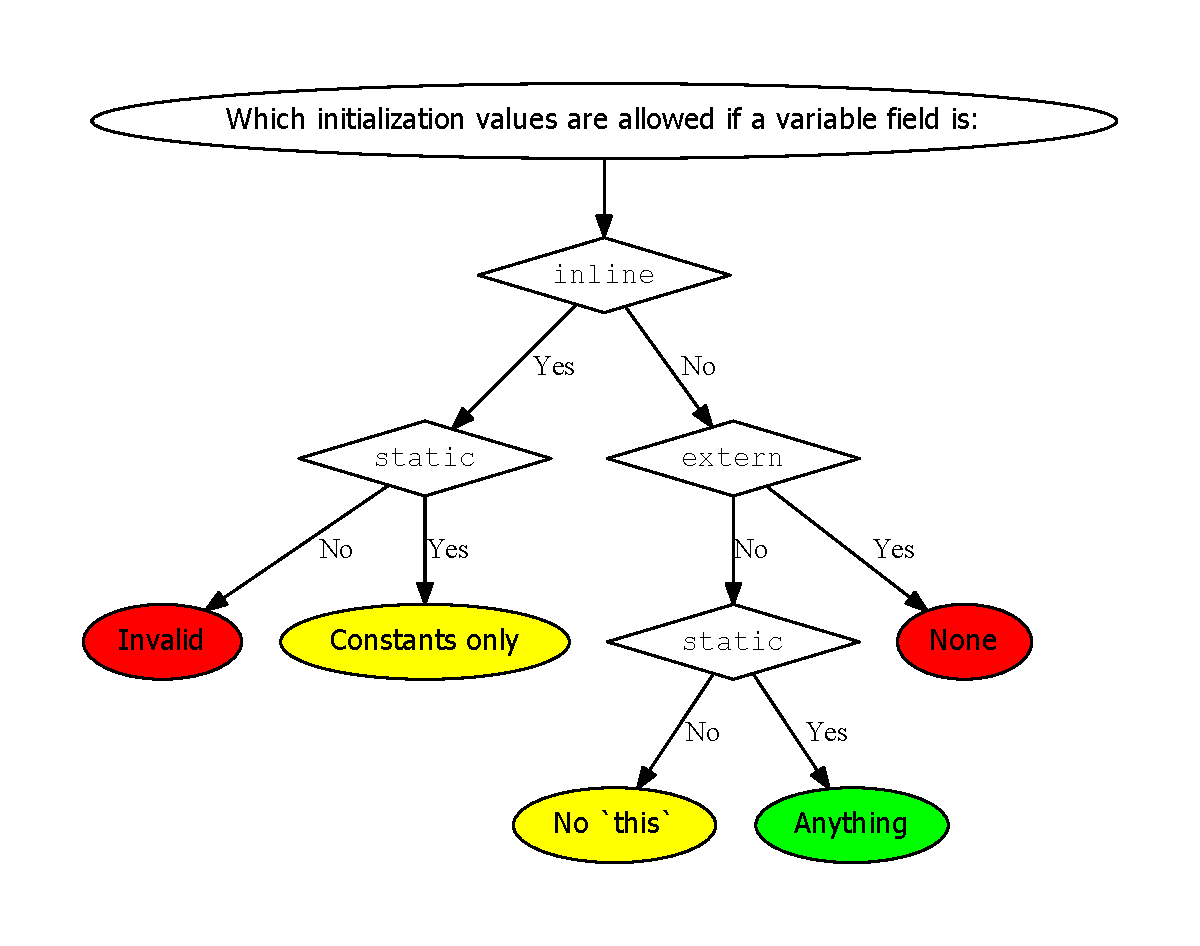
\includegraphics[width=1\textwidth]{assets/graphics/var-initialization.pdf}
	\caption{Variable initialization}
\end{figure}


\section{Property}
\label{class-field-property}

Next to \tref{variables}{class-field-variable}, properties are the second option for dealing with data on a class. Unlike variables however, they offer more control of which kind of field access should be allowed and how it should be generated. Common use cases include:

\begin{itemize}
	\item Have a field which can be read from anywhere, but only be written from within the defining class.
	\item Have a field which invokes a \emph{getter}-method upon read-access.
	\item Have a field which invokes a \emph{setter}-method upon write-access.
\end{itemize}

When dealing with properties, it is important to understand the two kinds of access:

\define{Read Access}{A read access to a field occurs when a right-hand side \tref{field access expression}{expression-field-access} is used. This includes calls in the form of \expr{obj.field()}, where \expr{field} is accessed to be read.}

\define{Write Access}{A write access to a field occurs when a \tref{field access expression}{expression-field-access} is assigned a value in the form of \expr{obj.field = value}. It may also occur in combination with \tref{read access}{def:Read Access} for special assignment operators such as \expr{+=} in expressions like \expr{obj.field += value}.} 

Read access and write access are directly reflected in the syntax, as the following example shows:

\haxe{assets/Property.hx}

For the most part, the syntax is similar to variable syntax, and the same rules indeed apply. Properties are identified by

\begin{itemize}
	\item the opening parenthesis \expr{(} after the field name,
	\item followed by a special \emph{access identifier} (here: \expr{default}),
	\item with a comma \expr{,} separating
	\item another special access identifier (here: \expr{null})
	\item before a closing parenthesis \expr{)}.
\end{itemize}

The access identifiers define the behavior when the field is read (first identifier) and written (second identifier). The accepted values are:

\begin{description}
	\item[\expr{default}:] Allows normal field access if the field has public visibility, otherwise equal to \expr{null} access.
	\item[\expr{null}:] Allows access only from within the defining class.
	\item[\expr{get}/\expr{set}:] Access is generated as a call to an \emph{accessor method}. The compiler ensures that the accessor is available.
	\item[\expr{dynamic}:] Like \expr{get}/\expr{set} access, but does not verify the existence of the accessor field.
	\item[\expr{never}:] Allows no access at all.
\end{description}

\define{Accessor method}{An \emph{accessor method} (or short \emph{accessor}) for a field named \expr{field} of type \type{T} is a \emph{getter} named \expr{get_field} of type \type{Void->T} or a \emph{setter} named \expr{set_field} of type \type{T->T}.}

\trivia{Accessor names}{In Haxe 2, arbitrary identifiers were allowed as access identifiers and would lead to custom accessor method names to be admitted. This made parts of the implementation quite tricky to deal with. In particular, \expr{Reflect.getProperty()} and \expr{Reflect.setProperty()} had to assume that any name could have been used, requiring the target generators to generate meta-information and perform lookups.\\
We disallowed these identifiers and went for the \expr{get_} and \expr{set_} naming convention which greatly simplified implementation. This was one of the breaking changes between Haxe 2 and 3.}

\subsection{Common accessor identifier combinations}
\label{class-field-property-common-combinations}

The next example shows common access identifier combinations for properties:

\haxe{assets/Property2.hx}

The \target{Javascript} output helps understand what the field access in the \expr{main}-method is compiled to:

\begin{lstlisting}
var Main = function() {
	var v = this.get_x();
	this.set_x(2);
	var _g = this;
	_g.set_x(_g.get_x() + 1);
};
\end{lstlisting}

As specified, the read access generates a call to \expr{get_x()}, while the write access generates a call to \expr{set_x(2)} where \expr{2} is the value being assigned to \expr{x}. The way the \expr{+=} is being generated might look a little odd at first, but can easily be justified by the following example:

\haxe{assets/Property3.hx}

What happens here is that the expression part of the field access to \expr{x} in the \expr{main} method is \emph{complex}: It has potential side-effects, such as the construction of \type{Main} in this case. Thus, the compiler cannot generate the \expr{+=} operation as \expr{new Main().x = new Main().x + 1} and has to cache the complex expression in a local variable:

\begin{lstlisting}
Main.main = function() {
	var _g = new Main();
	_g.set_x(_g.get_x() + 1);
}
\end{lstlisting}



\subsection{Impact on the type system}
\label{class-field-property-type-system-impact}

The presence of properties has several consequences on the type system. Most importantly, it is necessary to understand that properties are a compile-time feature and thus \emph{require the types to be known}. If we were to assign a class with properties to \type{Dynamic}, field access would \emph{not} respect accessor methods. Likewise, access restrictions no longer apply and all access is virtually public.

When using \expr{get} or \expr{set} access identifier, the compiler ensures that the getter and setter actually exists. The following problem does not compile:

\haxe{assets/Property4.hx}

The method \expr{get_x} is missing, but it need not be declared on the class defining the property itself as long as a parent class defines it:

\haxe{assets/Property5.hx}

The \expr{dynamic} access modifier works exactly like \expr{get} or \expr{set}, but does not check for the existence



\subsection{Rules for getter and setter}
\label{class-field-property-rules}

Visibility of accessor methods has no effect on the accessibility of its property. That is, if a property is \expr{public} and defined to have a getter, that getter may me defined as \expr{private} regardless.

Both getter and setter may access their physical field for data storage. The compiler ensures that this kind of field access does not go through the accessor method if made from within the accessor method itself, thus avoiding infinite recursion:

\haxe{assets/GetterSetter.hx}

However, the compiler assumes that a physical field exists only if at least one of the access identifiers is \expr{default} or \expr{null}.

\define{Physical field}{A field is considered to be \emph{physical} if it is either
	\begin{itemize}
		\item a \tref{variable}{class-field-variable}
		\item a \tref{property}{class-field-property} with the read-access or write-access identifier being \expr{default} or \expr{null}
		\item a \tref{property}{class-field-property} with \expr{:isVar} \tref{metadata}{lf-metadata}
	\end{itemize}
}

If this is not the case, access to the field from within an accessor method causes a compilation error:

\haxe{assets/GetterSetter2.hx}

If a physical field is indeed intended, it can be forced by attributing the field in question with the \expr{:isVar} \tref{metadata}{lf-metadata}:

\haxe{assets/GetterSetter3.hx}


\trivia{Property setter type}{It is not uncommon for new Haxe users to be surprised by the type of a setter being required to be \type{T->T} instead of the seemingly more natural \type{T->Void}. After all, why would a \emph{setter} have to return something?\\
The rationale is that we still want to be able to use field assignments using setters as right-side expressions. Given a chain like \expr{x = y = 1}, it is evaluated as \expr{x = (y = 1)}. In order to assign the result of \expr{y = 1} to \expr{x}, the former must have a value. If \expr{y} had a setter returning \type{Void}, this would not be possible.}


\section{Method}
\label{class-field-method}

While \tref{variables}{class-field-variable} hold data, methods are defining behavior of a program by hosting \tref{expressions}{expression}. We have seen method fields in every code example of this document with even the initial \tref{Hello World}{introduction-hello-world} example containing a \expr{main} method:

\haxe{assets/HelloWorld.hx}

Methods are identified by the \expr{function} keyword. We can also learn that they

\begin{enumerate}
	\item have a name (here: \expr{main}),
	\item have an argument list (here: empty \expr{()}),
	\item have a return type (here: \type{Void}),
	\item may have \tref{access modifiers}{class-field-access-modifier} (here: \expr{static} and \expr{public}) and
	\item may have an expression (here: \expr{\{trace(trace("Hello World");)\}}).
\end{enumerate}

We can also look at the next example to learn more about arguments and return types:

\haxe{assets/MethodField.hx}

Arguments are given by an opening parenthesis \expr{(} after the field name, a comma \expr{,} separated list of argument specifications and a closing parenthesis \expr{)}. Additional information on the argument specification is described in \Fullref{types-function}.

The example demonstrates how \tref{type inference}{type-system-type-inference} can be used for both argument and return types. The method \expr{myFunc} has two arguments but only explicitly gives the type of the first one, \expr{f}, as \type{String}. The second one, \expr{i}, is not type-hinted and it is left to the compiler to infer its type from calls made to it. Likewise, the return type of the method is inferred from the \expr{return true} expression as \type{Bool}.

\subsection{Overriding Methods}
\label{class-field-overriding}

Overriding fields is instrumental for creating class hierarchies. Many design patterns utilize it, but here we will explore only the basic functionality. In order to use overrides in a class, it is required that this class has a \tref{parent class}{types-class-inheritance}. Let us consider the following example:

\haxe{assets/Override.hx}

The important components here are

\begin{itemize}
	\item the class \type{Base} which has a field \expr{method} and a constructor,
	\item the class \type{Child} which \expr{extends Base} and also has a field \expr{method} being declared with \expr{override}, and
	\item the \type{Main} class whose \expr{main} method creates an instance of \expr{Child}, assigns it to a variable \expr{child} of explicit type \type{Base} and calls \expr{method()} on it.
\end{itemize}

The variable \expr{child} is explicitly typed as \type{Base} to highlight an important difference: At compile-time the type is known to be \type{Base}, but the runtime still finds the correct field \expr{method} on class \type{Child}. It is then obvious that the field access is resolved dynamically at runtime.

\subsection{Effects of variance and access modifiers}
\label{class-field-override-effects}

Overriding adheres to the rules of \tref{variance}{type-system-variance}. That is, their argument types allow \emph{contravariance} (less specific types) while their return type allows \emph{covariance} (more specific types):

\haxe{assets/OverrideVariance.hx}

Intuitively, this follows from the fact that arguments are ``written to'' the function and the return value is ``read from'' it.

The example also demonstrates how \tref{visibility}{class-field-visibility} may be changed: An overriding field may be \expr{public} if the overridden field is \expr{private}, but not the other way around.

It is not possible to override fields which are declared as \tref{\expr{inline}}{class-field-inline}. This is due to the conflicting concepts: While inlining is done at compile-time by replacing a call with the function body, overriding fields necessarily have to be resolved at runtime.
	
	
	
\section{Access Modifier}
\label{class-field-access-modifier}
\state{NoContent}

\subsection{Visibility}
\label{class-field-visibility}

Fields are by default \emph{private}, meaning that only the class and its sub-classes may access them. They can be made \emph{public} by using the \expr{public} access modifier, allowing access from anywhere.

\haxe{assets/Visibility.hx}

Access to field \expr{available} of class \type{MyClass} is allowed from within \type{Main} because it is denoted as being \expr{public}. However, while access to field \expr{unavailable} is allowed from within class \type{MyClass}, it is not allowed from within class \type{Main} because it is \expr{private} (explicitly, although this identifier is redundant here).

The example demonstrates visibility through \emph{static} fields, but the rules for member fields are equivalent. The following example demonstrates visibility behavior for when \tref{inheritance}{types-class-inheritance} is involved.

\haxe{assets/Visibility2.hx}

We can see that access to \expr{child1.baseField()} is allowed from within \type{Child2} even though \expr{child1} is of a different type, \type{Child1}. This is because the field is defined on their common ancestor class \type{Base}, contrary to field \expr{child1Field} which can not be accessed from within \type{Child2}.

Omitting the visibility modifier usually defaults the visibility to \expr{private}, but there are exceptions where it becomes \expr{public} instead:

\begin{enumerate}
	\item If the class is declared as \expr{extern}.
	\item If the field id declared on an \tref{interface}{types-interfaces}.
	\item If the field \tref{overrides}{class-field-overriding} a public field.
\end{enumerate}

\trivia{Protected}{Haxe has no notion of a \expr{protected} keyword known from Java, C++ and other object-oriented languages. However, its \expr{private} behavior is equal to those language's protected behavior, so Haxe actually lacks their real private behavior.}

\subsection{Inline}
\label{class-field-inline}

The \expr{inline} keyword allows function bodies to be directly inserted in place of calls to them. This can be a powerful optimization tool, but should be used judiciously as not all functions are good candidates for inline behavior. The following example demonstrates the basic usage:

\haxe{assets/Inline.hx}

The generated \target{Javascript} output reveals the effect of inline:

\begin{lstlisting}
(function () { "use strict";
var Main = function() { }
Main.main = function() {
	var a = 1;
	var b = 2;
	var c = (a + b) / 2;
}
Main.main();
})();
\end{lstlisting}

As evident, the function body \expr{s1 + s2} of field \expr{mid} was generated in place of the call to \expr{add(a, b)}, with \expr{s1} being replaced by \expr{a} and \expr{s2} being replaced by \expr{b}. This avoids a function call which, depending on the target and frequency of occurrences, may yield noticeable performance improvements.

It is not always easy to judge if a function qualifies for being inline. Short functions that have no writing expressions (such as a \expr{=} assignment) are usually a good choice, but even more complex functions can be candidates. However, in some cases inlining can actually be detrimental to performance, e.g. because the compiler has to create temporary variables for complex expressions.

\subsection{Dynamic}
\label{class-field-dynamic}

Methods can be denoted with the \expr{dynamic} keyword to make them (re-)bindable:

\haxe{assets/DynamicFunction.hx}

The first call to \expr{test()} invokes the original function which returns the \type{String} \expr{"original"}. In the next line, \expr{test} is \emph{assigned} a new function. This is precisely what \expr{dynamic} allows: Function fields can be assigned a new function. As a result, the next invocation of \expr{test()} returns the \type{String} \expr{"new"}.

Dynamic fields cannot be \expr{inline} for obvious reasons: While inlining is done at compile-time, dynamic functions necessarily have to be resolved at runtime.

%TODO: performance estimation %

\subsection{Override}
\label{class-field-override}

The access modifier \expr{override} is required when a field is declared which also exists on a \tref{parent class}{types-class-inheritance}. Its purpose is to ensure that the author of a class is aware of the override as this may not always be obvious in large class hierarchies. Likewise, having \expr{override} on a field which does not actually override anything (e.g. due to a misspelled field name) triggers an error as well.

The effects of overriding fields are detailed in \Fullref{class-field-overriding}. This modifier is only allowed on \tref{method}{class-field-method} fields.




\chapter{Expressions}
\label{expression}

Expressions in Haxe define what a program \emph{does}. Most expressions are found in the body of a \tref{method}{class-field-method}, where they are combined to express what that method should do. This section explains the different kinds of expressions. Some definitions help here:

\define{Name}{A general name may refer to
\begin{itemize}
	\item a type,
	\item a local variable,
	\item a local function or
	\item a field.
\end{itemize}}

\label{expression-rules}
\define{Identifier}{Haxe identifiers start with an underscore \expr{_}, a dollar \expr{\$}, a lower-case character \expr{a-z} or an upper-case character \expr{A-Z}. After that, any combination and number of \expr{_}, \expr{A-Z}, \expr{a-z} and \expr{0-9} may follow.\\
Further limitations follow from the usage context, which are checked upon typing:
\begin{itemize}
	\item Type names must start with an upper-case letter \expr{A-Z} or an underscore \expr{_}.
	\item Leading dollars are not allowed for any kind of \tref{name}{def:Name} (dollar-names are mostly used for \tref{macro reification}{macro-reification}).
\end{itemize}}


\section{Blocks}
\label{expression-block}

A block in Haxe starts with an opening curly brace \expr{\{} and ends with a closing curly brace \expr{\}}. A block may contain several expressions, each of which is followed by a semicolon \expr{;}. The general syntax is thus:

\begin{lstlisting}
{
	expr1;
	expr2;
	...
	exprN;
}
\end{lstlisting}
The value and by extension the type of a block-expression is equal to the value and the type of the last sub-expression.

Blocks can contain local variables declared by \tref{\expr{var} expression}{expression-var}, as well as local functions declared by \tref{\expr{function} expressions}{expression-function}. These are available within the block and within sub-blocks, but not outside the block. Also, they are available only after their declaration. The following example uses \expr{var}, but the same rules apply to \expr{function} usage:

\begin{lstlisting}
{
	a; // error, a is not declared yet
	var a = 1; // declare a
	a; // ok, a was declared
	{
		a; // ok, a is available in sub-blocks
	}
	a; // ok, a is still available after sub-blocks
}
a; // error, a is not available outside
\end{lstlisting}
At runtime, blocks are evaluated from top to bottom. Control flow (e.g. \tref{exceptions}{expression-try-catch} or \tref{return expressions}{expression-return}) may leave a block before all expressions 
are evaluated.


\section{Constants}
\label{expression-constants}

The Haxe syntax supports the following constants:

\begin{description}
	\item[Int:] An \tref{integer}{def:Int}, such as \expr{0}, \expr{1}, \expr{97121}, \expr{-12}, \expr{0xFF0000}.
	\item[Float:] A \tref{floating point number}{def:Float}, such as \expr{0.0}, \expr{1.}, \expr{.3}, \expr{-93.2}.
	\item[String:] A \tref{string of characters}{def:String}, such as \expr{""}, \expr{"foo"}, \expr{''}, \expr{'bar'}.
	\item[true,false:] A \tref{boolean}{def:Bool} value.
	\item[null:] The null value.
\end{description}

Furthermore, the internal syntax structure treats \tref{identifiers}{def:Identifier} as constants, which may be relevant when working with \tref{macros}{macro}.


\section{Binary Operators}
\label{expression-binops}

\section{Unary Operators}
\label{expression-unops}

\section{Array Declaration}
\label{expression-array-declaration}

Arrays are initialized by enclosing comma \expr{,} separated values in brackets \expr{[]}. A plain \expr{[]} represents the empty array, whereas \expr{[1, 2, 3]} initializes an array with three elements \expr{1}, \expr{2} and \expr{3}.

The generated code may be less concise on platforms that do not support array initialization. Essentially, such initialization code then looks like this:

\begin{lstlisting}
var a = new Array();
a.push(1);
a.push(2);
a.push(3);
\end{lstlisting}
This should be considered when deciding if a function should be \tref{inlined}{class-field-inline} as it may inline more code than visible in the syntax.

Advanced initialization techniques are described in \Fullref{lf-array-comprehension}.


\section{Object Declaration}
\label{expression-object-declaration}

Object declaration begins with an opening curly brace \expr{\{} after which \expr{key:value}-pairs separated by comma \expr{,} follow, and which ends in a closing curly brace \expr{\}}.

\begin{lstlisting}
{
	key1:value1,
	key2:value2,
	...
	keyN:valueN
}
\end{lstlisting}
Further details of object declaration are described in the section about \tref{anonymous structures}{types-anonymous-structure}.


\section{Field Access}
\label{expression-field-access}

Field access is expressed by using the dot \expr{.} followed by the name of the field.

\begin{lstlisting}
object.fieldName
\end{lstlisting}

This syntax is also used to access types within packages in the form of \expr{pack.Type}. 

The typer ensures that an accessed field actually exist and may apply transformations depending on the nature of the field. If a field access is ambiguous, understanding the \tref{resolution order}{type-systemresolution-order} may help.


\section{Function Call}
\label{expression-function-call}

Functions calls consist of an arbitrary subject expression followed by an opening parenthesis \expr{(}, a comma \expr{,} separated list of expressions as arguments and a closing parenthesis \expr{)}.

\begin{lstlisting}
subject(); // call with no arguments
subject(e1); // call with one argument
subject(e1, e2); // call with two arguments
subject(e1, ..., eN); // call with multiple arguments
\end{lstlisting}


\section{var}
\label{expression-var}

The \expr{var} keyword allows declaring multiple variables, separated by comma \expr{,}. Each variable has a valid \tref{identifier}{def:Identifier} and optionally a value assignment following the assignment operator \expr{=}. Variables can also have an explicit type-hint.

\begin{lstlisting}
var a; // declare local a
var b:Int; // declare variable b of type Int
var c = 1; // declare variable c, initialized to value 1
var d,e = 2; // declare variable d and variable e initialized to value 2
\end{lstlisting}

The scoping behavior of local variables is described in \Fullref{expression-block}.


\section{Local functions}
\label{expression-function}

Haxe supports first-class functions and allows declaring local functions in expressions. The syntax follows \tref{class field methods}{class-field-method}:

\haxe{assets/LocalFunction.hx}

We declare \expr{myLocalFunction} inside the \tref{block expression}{expression-block} of the \expr{main} class field. It takes one argument \expr{i} and adds it to \expr{value}, which is defined in the outside scope.

The scoping is equivalent to that of \tref{variables}{expression-var} and for the most part writing a named local function can be considered equal to assigning an unnamed local function to a local variable:

\begin{lstlisting}
var myLocalFunction = function(a) { }
\end{lstlisting}

However, there are some differences related to type parameters and the position of the function. We speak of a ``lvalue'' function if it is not assigned to anything upon its declaration, and an ``rvalue'' function otherwise.

\begin{itemize}
	\item Lvalue functions require a name and can have \tref{type parameters}{type-system-type-parameters}.
	\item Rvalue functions may have a name, but cannot have type parameters.
\end{itemize}


\section{new}
\label{expression-new}

The \expr{new} keyword signals that a \tref{class}{types-class-instance} or an \tref{abstract}{types-abstract} is being instantiated. It is followed by the \tref{type path}{def:Type path} of the type which is to be instantiated. It may also list explicit \tref{type parameters}{type-system-type-parameters} enclosed in \expr{<>} and separated by comma \expr{,}. After an opening parenthesis \expr{()} follow the constructor arguments, again separated by comma \expr{,}, with a closing parenthesis \expr{)} at the end.

\haxe{assets/New.hx}

Within the \expr{main} method we instantiate an instance of \type{Main} itself, with an explicit type parameter \type{Int} and the arguments \expr{12} and \expr{"foo"}. As we can see, the syntax is very similar to the \tref{function call syntax}{expression-function-call} and it is common to speak of ``constructor calls''.

\subsection{Inline constructors}
\label{expression-inline-constructor}
\since{3.1.0}

If a constructor is declared to be \tref{inline}{class-field-inline}, the compiler may try to optimize it away in certain situations. There are several requirements for this to work:

\begin{itemize}
	\item The result of the constructor call must be directly assigned to a local variable.
	\item The expression of the constructor field must only contain assignments to its fields.
\end{itemize}

The following example demonstrates constructor inlining:

\haxe{assets/NewInline.hx}

A look at the \target{Javascript} output reveals the effect:

\begin{lstlisting}
Main.main = function() {
	var pt_x = 1.2;
	var pt_y = 9.3;
};
\end{lstlisting}



\section{for}
\label{expression-for}

Haxe does not support traditional for-loops known from C. Its \expr{for} keyword expects an opening parenthesis \expr{(}, then a variable identifier followed by the keyword \expr{in} and an arbitrary expression used as iterating collection. After the closing parenthesis \expr{)} follows an arbitrary loop body expression.

\begin{lstlisting}
for (v in e1) e2;
\end{lstlisting}

The typer ensures that the type of \expr{e1} can be iterated over, which is typically the case if it has an \expr{iterator} method returning an \type{Iterator<T>}, or if it is an \type{Iterator<T>} itself.

Variable \expr{v} is then available within loop body \expr{e2} and holds the value of the individual elements of collection \expr{e1}.

The type of a \expr{for} expression is always \type{Void}, meaning it has no value and cannot be used as right-side expression.

The control flow of loops can be affected by \tref{\expr{break}}{expression-break} and \tref{\expr{continue}}{expression-continue} expressions.

\section{while}
\label{expression-while}

A normal while loop starts with the \expr{while} keyword, followed by an opening parenthesis \expr{(}, the condition expression and a closing paranthesis \expr{)}. After that follows the loop body expression:

\begin{lstlisting}
while(condition) expression;
\end{lstlisting}

The condition expression has to be of type \type{Bool}.

Upon each iteration, the condition expression is evaluated. If it evaluates to \expr{false}, the loop stops, otherwise it evaluates the loop body expression.

\haxe{assets/While.hx}

This kind of while-loop is not guaranteed to evaluate the loop body expression at all: If the condition does not hold from the start, it is never evaluated. This is different for \tref{do-while loops}{expression-do-while}.

\section{do-while}
\label{expression-do-while}

A do-while loop starts with the \expr{do} keyword followed by the loop body expression. After that follows the \expr{while} keyword, an opening parenthesis \expr{(}, the condition expression and a closing parenthesis \expr{)}:

\begin{lstlisting}
do expression while(condition);
\end{lstlisting}

The condition expression has to be of type \type{Bool}.

As the syntax suggests, the loop body expression is always evaluated at least once, unlike \tref{while}{expression-while} loops.

\section{if}
\label{expression-if}

Conditional expressions come in the form of a leading \expr{if} keyword, a condition expression enclosed in parentheses \expr{()} and a expression to be evaluated in case the condition holds:

\begin{lstlisting}
if (condition) expression;
\end{lstlisting}

The condition expression has to be of type \type{Bool}.

Optionally, \expr{expression} may be followed by the \expr{else} keyword as well as another expression to be evaluated if the condition does not hold:

\begin{lstlisting}
if (condition) expression1 else expression2;
\end{lstlisting}

Here, \expr{expression2} may consist of another \expr{if} expression:

\begin{lstlisting}
if (condition1) expression1
else if(condition2) expression2
else expression3
\end{lstlisting}

If the value of an \expr{if} expression is required, e.g. for \expr{var x = if(condition) expression1 else expression2}, the typer ensures that the types of \expr{expression1} and \expr{expression2} \tref{unify}{type-system-unification}. If no \expr{else} expression is given, the type is inferred to be \type{Void}.


\section{switch}
\label{expression-switch}

A basic switch expression starts with the \expr{switch} keyword and the switch subject expression, as well as the case expressions between curly braces \expr{\{\}}. Case expressions either start with the \expr{case} keyword and are followed by a pattern expression, or consist of the \expr{default} keyword. In both cases a colon \expr{:} and an optional case body expression follows:

\begin{lstlisting}
switch subject {
	case pattern1: case-body-expression-1;
	case pattern2: case-body-expression-2;
	default: default-expression;
}
\end{lstlisting}

Case body expressions never ``fall through'', so the \tref{\expr{break}}{expression-break} keyword is not supported in Haxe.

Switch expressions can be used as value; in that case the types of all case body expressions and the default expression must \tref{unify}{type-system-unification}.

Further details on syntax of pattern expressions are detailed in \Fullref{lf-pattern-matching}.

\section{try/catch}
\label{expression-try-catch}

\section{return}
\label{expression-return}

A \expr{return} expression can come with or without an value expression:

\begin{lstlisting}
return;
return expression;
\end{lstlisting}

It leaves the control-flow of the innermost function it is declared in, which has to be distinguished when \tref{local functions}{expression-function} are involved:

\begin{lstlisting}
function f1() {
	function f2() {
		return;
	}
	f2();
	expression;
}
\end{lstlisting}

The \expr{return} leaves local function \expr{f2}, but not \expr{f1}, meaning \expr{expression} is still evaluated.

If \expr{return} is used without a value expression, the typer ensures that the return type of the function it returns from is of \type{Void}. If it has a value expression, the typer \tref{unifies}{type-system-unification} its type with the return type (explicitly given or inferred by previous \expr{return} expressions) of the function it returns from.


\section{break}
\label{expression-break}

The \expr{break} keyword leaves the control flow of the innermost loop (\expr{for} or \expr{while}) it is declared in, stopping further iterations:

\begin{lstlisting}
while(true) {
	expression1;
	if (condition) break;
	expression2;
}
\end{lstlisting}

Here, \expr{expression1} is evaluated for each iteration, but as soon as \expr{condition} holds, \expr{expression2} is not evaluated anymore.

The typer ensures that it appears only within a loop. The \expr{break} keyword in \tref{\expr{switch} cases}{expression-switch} is not supported in Haxe.


\section{continue}
\label{expression-continue}

The \expr{continue} keyword ends the current iteration of the innermost loop (\expr{for} or \expr{while}) it is declared in, causing the loop condition to be checked for the next iteration:

\begin{lstlisting}
while(true) {
	expression1;
	if(condition) continue;
	expression2;
}
\end{lstlisting}

Here, \expr{expression1} is evaluated for each iteration, but if \expr{condition} holds, \expr{expression2} is not evaluated for the current iteration. Unlike \expr{break}, iterations continue.

The typer ensures that it appears only within a loop.


\section{throw}
\label{expression-throw}

\section{cast}
\label{expression-cast}





\chapter{Language Features}
\label{lf}
\state{NoContent}

\section{Conditional Compilation}
\label{lf-condition-compilation}

Haxe allows conditional compilation by using \expr{\#if}, \expr{\#elseif} and \expr{\#else} and checking for \emph{compiler flags}.

\define{Compiler Flag}{A compiler flag is a configurable value which may influence the compilation process. Such a flag can be set by invoking the command line with \expr{-D key=value} or just \expr{-D key}, in which case the value defaults to \expr{"1"}. The compiler also sets several flags internally to pass information between different compilation steps.}

This example demonstrates usage of conditional compilation:

\haxe{assets/ConditionalCompilation.hx}

Compiling this without any flags will leave only the \expr{trace("ok");} line in the body of the \expr{main} method. The other branches are discarded while parsing the file. As a consequence, these branches must still contain valid Haxe syntax, but the code is not type-checked.

The conditions after \expr{\#if} and \expr{\#elseif} allow the following expressions:

\begin{itemize}
	\item Any identifier is replaced by the value of the compiler flag by the same name. Note that \expr{-D some-flag} from command line leads to the flags \expr{some-flag} and \expr{some\_flag} to be defined.
	\item The values of \type{String}, \type{Int} and \type{Float} constants are used directly.
	\item The boolean operators \expr{\&\&} (and), \expr{||} (or) and \expr{!} (not) work as expected.
	\item The operators \expr{==}, \expr{!=}, \expr{>}, \expr{>=}, \expr{<}, \expr{<=} can be used to compare values.
	\item Parentheses \expr{()} can be used to group expressions as usual.
\end{itemize}

An exhaustive list of all built-in defines can be obtained by invoking the Haxe Compiler with the \expr{--help-defines} argument. The Haxe Compiler allows multiple \expr{-D} flags per compilation.


\section{Externs}
\label{lf-externs}

Externs can be used to describe target-specific interaction in a type-safe manner. They are defined like normal classes, except that

\begin{itemize}
	\item the \expr{class} keyword is preceded by the \expr{extern} keyword,
	\item \tref{methods}{class-field-method} have no expressions and
	\item all argument and return types are explicit.
\end{itemize}

A common example from the \tref{Haxe Standard Library}{std} is the \type{Math} class, as an excerpt shows:

\begin{lstlisting}
extern class Math
{
	static var PI(default,null) : Float;
	static function floor(v:Float):Int;
}
\end{lstlisting}

We see that externs can define both methods and variables (actually, \expr{PI} is declared as a read-only \tref{property}{class-field-property}). Once this information is available to the compiler, it allows field access accordingly and also knows the types:

\haxe{assets/Extern.hx}

This works because the return type of method \expr{floor} is declared to be \type{Int}.

The Haxe Standard Library comes with many externs for the \target{Flash} and \target{Javascript} target. They allow accessing the native APIs in a type-safe manner and are instrumental for designing higher-level APIs. There are also externs for many popular native libraries on \tref{haxelib}{haxelib}.

The \target{Flash}, \target{Java} and \target{C\#} targets allow direct inclusion of native libraries from \tref{command line}{compiler-reference}. Target-specific details are explained in the respective sections of \Fullref{target-details}.




\section{Static Extension}
\label{lf-static-extension}

\define{Static Extension}{A static extension allows pseudo-extending existing types without modifying their source. In Haxe this is achieved by declaring a static method with a first argument of the extending type and then bringing the defining class into context through \expr{using}.}

Static extensions can be a powerful tool which allows augmenting types without actually changing them. The following example demonstrates the usage:

\haxe{assets/StaticExtension.hx}

Clearly, \type{Int} does not natively provide a \expr{triple} method, yet this program compiles and outputs \expr{36} as expected. This is because the call to \expr{12.triple()} is transformed into \expr{IntExtender.triple(12)}. There are three requirements for this:

\begin{enumerate}
	\item Both the literal \expr{12} and the first argument of \expr{triple} are of type \type{Int}.
	\item The class \type{IntExtender} is brought into context through \expr{using Main.IntExtender}.
	\item \type{Int} does not have a \expr{triple} field by itself (if it had, that field would take priority over the static extension).
\end{enumerate}

Static extensions are usually considered syntactic sugar and indeed they are, but it is worth noting that they can have a dramatic effect on code readability: Instead of nested calls in the form of \expr{f1(f2(f3(f4(x))))}, chained calls in the form of \expr{x.f4().f3().f2().f1()} can be used.

Following the rules previously described in \Fullref{type-systemresolution-order}, multiple \expr{using} expressions are checked from bottom to top, with the types within each module as well as the fields within each type being checked from top to bottom. Using a module (as opposed to a specific type of a module, see \Fullref{type-system-modules-and-paths}) as static extension brings all its types into context.

\subsection{In the Haxe Standard Library}
\label{lf-static-extension-in-std}

Several classes in the Haxe Standard Library are suitable for static extension usage. The next example shows the usage of \type{StringTools}:

\haxe{assets/StaticExtension2.hx}

While \type{String} does not have a \expr{replace} functionality by itself, the \expr{using StringTools} static extension provides one. As usual, the \target{Javascript} output nicely shows the transformation:

\begin{lstlisting}
Main.main = function() {
	StringTools.replace("adc","d","b");
}
\end{lstlisting}

The following classes from the Haxe Standard Library are designed to be used as static extensions:

\begin{description}
	\item[\type{StringTools}:] Provides extended functionality on strings, such as replacing or trimming.
	\item[\type{Lambda}:] Provides functional methods on iterables.
	\item[\type{haxe.EnumTools}:] Provides type information functionality on enums and their instances.
	\item[\type{haxe.macro.Tools}:] Provides different extensions for working with macros (see \Fullref{macro-tools}).
\end{description}



\trivia{``using'' using}{Since the \expr{using} keyword was added to the language, it has been common to talk about certain problems with ``using using'' or the effect of ``using using''. This makes for awkward English in many cases, so the author of this manual decided to call the feature by what it actually is: Static extension.}



\section{Pattern Matching}
\label{lf-pattern-matching}
\state{NoContent}
\todo{Check ``you'' wording.}

\subsection{Introduction}
\label{lf-pattern-matching-introduction}

Haxe 3 comes with improved options for pattern matching. Here we will explore the syntax for different patterns using this data structure as running example:

\haxe[firstline=1,lastline=4]{assets/PatternMatching.hx}

Some pattern matcher basics include:

\begin{itemize}
	\item Patterns will always be matched from top to bottom.
	\item The topmost pattern that matches the input value has its expression executed.
	\item A \expr{_} pattern matches anything, so \expr{case _}: is equal to \expr{default:}
\end{itemize}

\subsection{Enum matching}
\label{lf-pattern-matching-enums}

As with Haxe 2, enums can be matched by their constructors in a natural way. With Haxe 3 pattern matching, this match can now be "deep":

\haxe[firstline=8,lastline=19]{assets/PatternMatching.hx}

The pattern matcher will check each case from top to bottom and pick the first one that matches the input value. If you are not too familiar with pattern matching, the following manual interpretation of each case rule might help:

\begin{description}
	\item[\expr{case Leaf(_)}:] matching fails because \expr{myTree} is a \expr{Node}
	\item[\expr{case Node(_, Leaf(_))}:] matching fails because the right sub-tree of \expr{myTree} is not a \expr{Leaf}, but another \expr{Node}
	\item[\expr{case Node(_, Node(Leaf("bar"), _))}:] matching succeeds
	\item[\expr{case _}:] this is not checked here because the previous line matched
\end{description}

\subsection{Variable capture}
\label{lf-pattern-matching-variable-capture}

It is possible to catch any value of a sub-pattern by matching it against an identifier:

\haxe[firstline=22,lastline=28]{assets/PatternMatching.hx}

This would return one of the following:

\begin{itemize}
	\item If \expr{myTree} is a \expr{Leaf}, its name is returned.
	\item If \expr{myTree} is a \expr{Node} whose left sub-tree is a \expr{Leaf}, its name is returned (this will apply here, returning \expr{"foo"}).
	\item Otherwise \expr{"none"} is returned.
\end{itemize}

It is also possible to use = to capture values which are further matched:

\haxe[firstline=30,lastline=34]{assets/PatternMatching.hx}

Here, \expr{leafNode} is bound to \expr{Leaf("foo")} if the input matches that. In all other cases, \expr{myTree} itself is returned: \expr{case x} works similar to \expr{case _} in that it matches anything, but with an identifier name like \expr{x} it also binds the matched value to that variable.

\subsection{Structure matching}
\label{lf-pattern-matching-structure}

It is now also possible to match against the fields of anonymous structures and instances:

\haxe[firstline=36,lastline=42]{assets/PatternMatching.hx}

Note that in the second case, we bind the matched \expr{name} field to identifier \expr{n} if \expr{rating} matches \expr{"awesome"}. Of course you could also put this structure into the \type{Tree} from the previous example and combine structure and enum matching.

A limitation with regards to class instances is that you cannot match against fields of their parent class.

\subsection{Array matching}
\label{lf-pattern-matching-array}

Arrays can be matched on fixed length:

\haxe[firstline=45,lastline=53]{assets/PatternMatching.hx}

This will trace \expr{1} because \expr{array[1]} matches \expr{6}, and \expr{array[0]} is allowed to be anything.

\subsection{Or patterns}
\label{lf-pattern-matching-or}

The \expr{|} operator can be used anywhere within patterns to describe multiple accepted patterns:

\haxe[firstline=56,lastline=61]{assets/PatternMatching.hx}

If there's a captured variable in an or-pattern, it must appear in both its sub-patterns.

\subsection{Guards}
\label{lf-pattern-matching-guards}

It is also possible to further restrict patterns with the \expr{case ... if(condition):} syntax:

\haxe[firstline=64,lastline=72]{assets/PatternMatching.hx}

Note how the first case has an additional guard condition \expr{if (b > a)}. It will only be selected if that condition holds, otherwise matching continues with the next case.

\subsection{Match on multiple values}
\label{lf-pattern-matching-tuples}

Array syntax can also be used to match on multiple values:

\haxe[firstline=75,lastline=80]{assets/PatternMatching.hx}

This is quite similar to usual array matching, but there are differences:

\begin{itemize}
	\item The number of elements is fixed, so patterns of different array length will not be accepted.
	\item It is not possible to capture the switch value in a variable, i.e. \expr{case x} is not allowed (\expr{case _} still is).
\end{itemize}




\subsection{Extractors}
\label{lf-pattern-matching-extractors}
\since{3.1.0}

Extractors allow applying transformations to values being matched. This is often useful when a small operation is required on a matched value before matching can continue:

\haxe{assets/Extractor2.hx}

Here we have to capture the argument value of the \expr{TString} enum constructor in a variable \expr{temp} and use a nested switch on \expr{temp.toLowerCase()}. Obviously, we want matching to succeed if \expr{TString} holds a value of \expr{"foo"} regardless of its casing. This can be simplified with extractors:

\haxe{assets/Extractor.hx}

Extractors are identified by the \expr{extractorExpression => match} expression. The compiler generates code which is similar to the previous example, but the original syntax was greatly simplified. The way extractors are treated depends on the expression left of the \expr{=>} operator. If it is

\begin{itemize}
	\item any identifier \expr{i}, the generated code is equal to \expr{matchedValue.i()},
	\item otherwise for arbitrary expressions \expr{e}, it is equal to \expr{e(matchedValue)}.
\end{itemize}

The distinction is made because interpreting a plain identifier like that can be quite convenient, as the \expr{toLowerCase()} example above demonstrated. It also allows bringing extractors into context through \tref{static extensions}{lf-static-extension}.

Any expression can be used as extractor expression and the typer ensures that it is of function type \type{S->T}, where \type{S} is the type of the currently matched value and \type{T} is equal to the type of the expression right of the \expr{=>} operator. With that, extractors can be combined with other features such as \tref{function binding}{lf-function-bindings}:

\haxe{assets/Extractor3.hx}

In this particular case, the extractor is called as \expr{lessThan(4, 5)}, yielding true.

A lcurrent imitation with regards to extractors is that they disable \tref{useless pattern checks}{lf-pattern-matching-unused}.


\subsection{Exhaustiveness checks}
\label{lf-pattern-matching-exhaustiveness}

The compiler ensures that you do not forget a possible case for non value-only switches:

\begin{lstlisting}
switch(true) {
    case false:
} // This match is not exhaustive, these patterns are not matched: true
\end{lstlisting}

The matched type \type{Bool} admits two values \expr{true} and \expr{false}, but only \expr{false} is checked. 


\subsection{Useless pattern checks}
\label{lf-pattern-matching-unused}

In a similar fashion, the compiler detects patterns which will never match the input value:

\begin{lstlisting}
switch(Leaf("foo")) {
    case Leaf(_)
       | Leaf("foo"): // This pattern is unused
    case Node(l,r):
    case _: // This pattern is unused
}
\end{lstlisting}



\section{String Interpolation}
\label{lf-string-interpolation}

With Haxe 3 it is no longer necessary to manually concatenate parts of a string due to the introduction of \emph{String Interpolation}. Special identifiers, denoted by the dollar sign \expr{\$} within a String enclosed by single-quote \expr{'} characters, are evaluated as if they were concatenated identifiers:

\begin{lstlisting}
var x = 12;
trace('The value of x is $x'); // The value of x is 12
\end{lstlisting}
Furthermore, it is possible to include whole expressions in the string by using \expr{\$$\left\{expr\right\}$}, with \expr{expr} being any valid Haxe expression:

\begin{lstlisting}
var x = 12;
trace('The sum of $x and 3 is ${x + 3}'); // The sum of 12 and 3 is 15
\end{lstlisting} 
String interpolation is a compile-time feature and has no impact on the runtime. The above example is equivalent to manual concatenation, which is exactly what the compiler generates:

\begin{lstlisting}
trace("The sum of " +x+ " and 3 is " + (x + 3));
\end{lstlisting}
Of course the use of single-quote enclosed strings without any interpolation remains valid, but care has to be taken regarding the \$ character as it triggers interpolation. If an actual dollar-sign should be used in the string, \expr{\$\$} can be used.

\trivia{String Interpolation before Haxe 3}{String Interpolation has been a Haxe feature since version 2.09. Back then, the macro \expr{Std.format} had to be used, being both slower and less comfortable than the new string interpolation syntax.}


\section{Array Comprehension}
\label{lf-array-comprehension}

Array comprehension in Haxe uses existing syntax to allow concise initialization of arrays. It is identified by \expr{[for} or \expr{[while} constructs:

\haxe{assets/ArrayComprehension.hx}

Variable \expr{a} is initialized to an array holding the numbers 0 to 9. The compiler generates code which adds the value of each loop iteration to the array, so the following code would be equivalent:

\begin{lstlisting}
var a = [];
for (i in 0...10) a.push(i);
\end{lstlisting}

Variable \expr{b} is initialized to an array with the same values, but through a different comprehension style using \expr{while} instead of \expr{for}. Again, the following code would be equivalent:

\begin{lstlisting}
var i = 0;
var a = [];
while(i < 10) a.push(i++);
\end{lstlisting}

The loop expression can be anything, including conditions and nested loops, so the following works as expected:

\haxe{assets/AdvArrayComprehension.hx}


\section{Iterators}
\label{lf-iterators}

With Haxe it is very easy to define custom iterators and iterable data types. These concepts are represented by the types \type{Iterator<T>} and \type{Iterable<T>} respectively:

\begin{lstlisting}
typedef Iterator<T> = {
	function hasNext() : Bool;
	function next() : T;
}

typedef Iterable<T> = {
	function iterator() : Iterator<T>;
}
\end{lstlisting}

Any \tref{class}{types-class-instance} which \tref{structurally unifies}{type-system-structural-subtyping} with one of these types can be iterated over using a \tref{for-loop}{expression-for}. That is, if the class defines methods \expr{hasNext} and \expr{next} with matching return types it is considered an iterator, if it defines a method \expr{iterator} returning an \type{Iterator<T>} it is considered an iterable type.

\haxe{assets/Iterator.hx}

The type \type{MyStringIterator} in this example qualifies as iterator: It defines a method \expr{hasNext} returning \type{Bool} and a method \expr{next} returning \type{String}, making it compatible with \type{Iterator<String>}. The \expr{main} method instantiates it, then iterates over it.

\haxe{assets/Iterable.hx}

Here we do not setup a full iterator like in the previous example, but instead define that the \type{MyArrayWrap<T>} has a method \expr{iterator}, effectively forwarding the iterator method of the wrapped \type{Array<T>} type. 



\section{Function Bindings}
\label{lf-function-bindings}

Haxe 3 allows binding functions with partially applied arguments. Each function type can be considered to have a \expr{bind} field, which can be called with the desired number of arguments in order to create a new function. This is demonstrated here:

\haxe{assets/Bind.hx}
Line 4 binds the function \expr{map.set} to a variable named \expr{f}, and applies \expr{12} as second argument. The underscore \expr{_} is used to denote that this argument is not bound, which is shown by comparing the types of \expr{map.set} and \expr{f}: The bound \type{String} argument is effectively cut from the type, turning a \expr{Int->String->Void} type into \expr{Int->Void}.

A call to \expr{f(1)} then actually invokes \expr{map.set(1, "12")}, the calls to \expr{f(2)} and \expr{f(3)} are analogous. The last line proves that all three indices indeed are mapped to the value \expr{"12"}.

The underscore \expr{_} can be skipped for trailing arguments, so the the first argument could be bound through \expr{map.set.bind(1)}, yielding a \expr{String->Void} function that sets a new value for index \expr{1} on invocation.

\trivia{Callback}{Prior to Haxe 3, Haxe used to know a \expr{callback}-keyword which could be called with a function argument followed by any number of binding arguments. The name originated from a common usage were a callback-function is created with the this-object being bound.\\
Callback would allow binding of arguments only from left to right as there was no support for the underscore \expr{_}. The choice to use an underscore was controversial and several other suggestions were made, none of which were considered superior. After all, the underscore \expr{_} at least looks like it's saying ``fill value in here'', which nicely describes its semantics.}



\section{Metadata}
\label{lf-metadata}

Several constructs can be attributed with custom metadata:

\begin{itemize}
	\item \expr{class} and \expr{enum} declarations
	\item Class fields
	\item Enum constructors
	\item Expressions
\end{itemize}

These metadata information can be obtained at runtime through the \type{haxe.rtti.Meta} API:

\haxe{assets/Meta.hx}

We can easily identify metadata by the leading \expr{@} character, followed by the metadata name and, optionally, by a number of comma-separated constant arguments enclosed in parentheses.

\begin{itemize}
	\item Class \type{MyClass} has an \expr{author} metadata with a single String argument \expr{"Nicolas"}, as well as a \expr{debug} metadata without arguments.
	\item The member variable \expr{value} has a \expr{range} metadata with two Int arguments \expr{1} and \expr{8}.
	\item The static method \expr{method} has a \expr{broken} metadata without arguments, as well as a \expr{:noCompletion} metadata without arguments.
\end{itemize}

The \expr{main} method accesses these metadata values using their API. The output reveals the structure of the obtained data:

\begin{itemize}
	\item There is a field for each metadata, with the field name being the metadata name.
	\item The field values correspond to the metadata arguments. If there are no arguments, the field value is \expr{null}. Otherwise the field value is an array with one element per argument.
	\item Metadata starting with \expr{:} is omitted. This kind of metadata is known as \emph{compiler metadata}.
\end{itemize}

Allowed values for metadata arguments are:

\begin{itemize}
	\item \tref{Constants}{expression-constants}
	\item \tref{Arrays declarations}{expression-array-declaration} (if all their elements qualify)
	\item \tref{Object declarations}{expression-object-declaration} (if all their field values qualify)
\end{itemize}

\section{Access Control}
\label{lf-access-control}

Access control can be used if the basic \tref{visibility}{class-field-visibility} options are not sufficient. It is applicable at \emph{class-level} and at \emph{field-level} and knows two directions:

\begin{description}
	\item[Allowing access:] The target is granted access to the given class or field by using the \expr{:allow(target)} \tref{metadata}{lf-metadata}.
	\item[Forcing access:] A target is forced to allow access to the given class or field by using the \expr{:access(target)} \tref{metadata}{lf-metadata}.
\end{description}

In this context, a \emph{target} can be the \tref{dot-path}{def:Type path} to

\begin{itemize}
	\item a \emph{class field},
	\item a \emph{class} or \emph{abstract} type, or
	\item a \emph{package}.
\end{itemize}

If it is a class or abstract type, access modification extends to all fields of that type. Likewise, if it is a package, access modification extends to all types of that package and recursively to all fields of these types.

\haxe{assets/ACL.hx}

Here, \expr{MyClass.foo} can be accessed from the \expr{main}-method because \type{MyClass} is annotated with \expr{@:allow(Main)}. This would also work with \expr{@:allow(Main.main)} and both versions could alternatively be annotated to the field \expr{foo} instead of the class \type{MyClass}:

\haxe{assets/ACL2.hx}

If a type cannot be modified to allow this kind of access, the accessing method may force access:

\haxe{assets/ACL3.hx}

The \expr{@:access(MyClass.foo)} annotation effectively subverts the visibility of the \expr{foo} field within the \expr{main}-method. 

\trivia{On the choice of metadata}{The access control language feature uses the Haxe metadata syntax instead of additional language-specific syntax. There are several reasons for that:\\
\begin{itemize}
	\item Additional syntax often adds complexity to the language parsing, and also adds (too) many keywords.
	\item Additional syntax requires additional learning by the language user, whereas metadata syntax is something that is already known.
	\item The metadata syntax is flexible enough to allow extension of this feature.
	\item The metadata can be accessed/generated/modified by Haxe macros.
\end{itemize}
Of course, the main drawback of using metadata syntax is that you get no error report in case you misspell either the metadata key (@:acesss for instance) or the class/package name. However, with this feature you will get an error when you try to access a private field that you are not allowed to, therefore there is no possibility for silent errors.}

\since{3.1.0}

If access is allowed to an \tref{interface}{types-interfaces}, it extends to all classes implementing that interface:

\haxe{assets/ACL4.hx}

This is also true for access granted to parent classes, in which case it extends to all child classes.

\trivia{Broken feature}{Access extension to child classes and implementing classes was supposed to work in Haxe 3.0 and even documented accordingly. While writing this manual it was found that this part of the access control implementation was simply missing.}


\section{Remoting}
\label{lf-remoting}

\section{Runtime Type Information}
\label{lf-rtti}

\part{Compiler Reference}

\chapter{Compiler Reference}
\label{compiler-reference}

\section{Compiler Metadata}
\label{cr-metadata}

\chapter{Compiler Features}
\label{cr-features}
\state{NoContent}

\section{Dead Code Elimination}
\label{cr-dce}

Dead Code Elimination, or \emph{DCE}, is a compiler feature which removes unused code from the output. After typing, the compiler evaluates the DCE entry-points (usually the main-method) and recursively determines which fields and types are used. Used fields are marked accordingly and unmarked fields are then removed from their classes.

DCE has three modes which are set when invoking the command line:

\begin{description}
	\item[-dce std:] Only classes in the Haxe Standard Library are affected by DCE. This is the default setting on all targets but \target{Javascript}.
	\item[-dce no:] No DCE is performed.
	\item[-dce full:] All classes are affected by DCE. This is the default setting when targeting \target{Javascript}.
\end{description}
The DCE-algorithm works well with typed code, but may fail when \tref{dynamic}{types-dynamic} or \tref{reflection}{std-reflection} is involved. This may require explicit marking of fields or classes as being used by attributing the following metadata:

\begin{description}
	\item[\expr{@:keep}:] If used on a class, the class along with all fields is unaffected by DCE. If used on a field, that field is unaffected by DCE.
	\item[\expr{@:keepSub}:] If used on a class, it works like \expr{@:keep} on the annotated class as well as all subclasses.
	\item[\expr{@:keepInit}:] Usually, a class which had all fields removed by DCE (or is empty to begin with) is removed from the output. By using this metadata, empty classes are kept.
\end{description}
The compiler automatically defines the flag \expr{dce} with a value of either \expr{"std"}, \expr{"no"} or \expr{"full"} depending on the active mode. This can be used in \tref{conditional compilation}{lf-condition-compilation}.

\trivia{DCE-rewrite}{DCE was originally implemented in Haxe 2.07. This implementation considered a function to be used when it was explicitly typed. The problem with that was that several features, most importantly interfaces, would cause all class fields to be typed in order to verify type-safety. This effectively subverted DCE completely, prompting the rewrite for Haxe 2.10.}

\trivia{DCE and try.haxe.org}{DCE for the \type{Javascript} target saw vast improvements when the website \url{http://try.haxe.org} was published. Initial reception of the generated \target{Javascript} code was mixed, leading to a more fine-grained selection of which code to eliminate.}

\section{Completion}
\label{cr-completion}

\subsection{Field Access}
\label{Field access}

\subsection{Call Arguments}
\label{Call arguments}

\subsection{Usage}
\label{usage}

\subsection{Position}
\label{position}

\subsection{Metadata}
\label{metadata}

\section{Resources}
\label{cr-resources}

Haxe provides simple resource embedding system that can be used for embedding  files directly into the compiled application.

While it may be not optimal to embed large assets, like images or music in the application file, it comes in very handy to embed smaller resources, like configuration or XML data.

\subsection{Embedding resources}
\label{cr-resources-embed}

External files are embedded using the \emph{-resource} compiler argument:

\todo{what to use for listing of non-haxe code like hxml?}
\begin{lstlisting}
-resource hello_message.txt@welcome
\end{lstlisting}

The string after the \emph{@} symbol is the \emph{resource identifier}. It will used in the code for retrieving the resource. It can be omitted (together with the \emph{@} symbol), then the file name will become a resource identifier.

\subsection{Retrieving text resources}
\label{cr-resources-getString}

To retrieve the content of an embedded resource, we use the static method \emph{getString} of \type{haxe.Resource} passing a \emph{resource identifier} to it:

\haxe{assets/ResourceGetString.hx}

The code above will display the content of the \emph{hello_message.txt} file that we included earlier using \emph{welcome} as the identifier.

\subsection{Retrieving binary resources}
\label{cr-resources-getBytes}

While it's not recommended to embed large binary files in the application, it still may be useful to embed binary data. Binary representation of an embedded resource can be accessed using the static method \emph{getBytes} of \type{haxe.Resource}:

\haxe{assets/ResourceGetBytes.hx}

The return type of \emph{getBytes} method is \type{haxe.io.Bytes}, an object providing access to individual bytes of the data.

\subsection{Implementation details}
\label{cr-resources-impl}

\todo{do we need to describe this?}
Haxe uses target platform's native resource embedding, if there is one, providing its own implementation otherwise.

\begin{itemize}
\item \emph{Flash} resources are embedded as ByteArray definitions
\item \emph{C\#} resources are included in the compiled assembly
\item \emph{Java} resources are packed in the resulting JAR file
\item \emph{C++} resources are stored in global byte array constants.
\item \emph{JavaScript} resources are serialized in Haxe serialization format and stored in a static field of \type{haxe.Resource} class.
\item \emph{Neko} resources are stored as strings in a static field of \type{haxe.Resource} class.
\end{itemize}

\chapter{Macros}
\label{macro}

Macros are without a doubt the most advanced feature in Haxe. They are often perceived as dark magic that only a select few are capable of mastering, yet there is nothing magical (and certainly nothing dark) about them.

\define{Abstract Syntax Tree (AST)}{The AST is the result of \emph{parsing} Haxe code into a typed structure. This structure is exposed to macros through the types defined in the file \expr{haxe/macro/Expr.hx} of the Haxe Standard Library.}

A basic macro is a \emph{syntax-transformation}. It receives zero or more \tref{expressions}{expression} and also returns an expression. If a macro is called, it effectively inserts code at the place it was called from. In that respect, it could be compared to a preprocessor like \expr{\#define} in C++, but a Haxe macro is not a textual replacement tool.

We can identify different kinds of macros, which are run at specific compilation stages:

\begin{description}
	\item[Initialization Macros:] These are provided by command line using the \ic{--macro} compiler parameter. They are executed after the compiler arguments were processed and the \emph{typer context} has been created, but before any typing was done (see \Fullref{macro-compiler-configuration}).
	\item[Build Macros:] These are defined for classes, enums and abstracts through the \expr{@:build} or \expr{@:autoBuild} \tref{metadata}{lf-metadata}. They are executed per-type, after the type has been set up (including its relation to other types, such as inheritance for classes) but before its fields are typed (see \Fullref{macro-type-building}).
	\item[Expression Macros:] These are normal functions which are executed as soon as they are typed.
\end{description}
	
\section{Macro Context}
\label{macro-context}

\define{Macro Context}{The macro context is the environment in which the macro is executed. Depending on the macro type, it can be considered to be a class being built or a function being typed. Contextual information can be obtained through the \ic{haxe.macro.Context} API.}

Haxe macros have access to different contextual information depending on the macro type. Other than querying such information, the context also allows some modifications such as defining a new type or registering certain callbacks. It is important to understand that not all information is available for all macro kinds, as the following examples demonstrate:

\begin{itemize}
	\item Initialization macros will find that the \expr{Context.getLocal*()} methods return \expr{null}. There is no local type or method in the context of an initialization macro.
	\item Only build macros get a proper return value from \expr{Context.getBuildFields()}. There are no fields being built for the other macro kinds.
	\item Build macros have a local type (if incomplete), but no local method, so \expr{Context.getLocalMethod()} returns \expr{null}.
\end{itemize}

The context API is complemented by the \expr{haxe.macro.Compiler} API detailed in \Fullref{macro-compiler-configuration}. While this API is available to all macro kinds, care has to be taken for any modification outside of initialization macros. This stems from the natural limitation of undefined \tref{build order}{macro-limitations-build-order}, which could cause e.g. a flag definition through \expr{Compiler.define()} to take effect before or after a \tref{conditional compilation}{lf-condition-compilation} check against that flag.

\section{Arguments}
\label{macro-arguments}

Most of the time, arguments to macros are expressions represented as an instance of enum \type{Expr}. As such, they are parsed but not typed, meaning they can be anything conforming to Haxe's syntax rules. The macro can then inspect their structure, or (try to) get their type using \expr{haxe.macro.Context.typeof()}.

It is important to understand that arguments to macros are not guaranteed to be evaluated, so any intended side-effect is not guaranteed to occur. On the other hand, it is also important to understand that an argument expression may be duplicated by a macro and used multiple times in the returned expression:

\haxe{assets/MacroArguments.hx}

The macro \expr{add} is called with \expr{x++} as argument and thus returns \expr{x++ + x++} using \tref{expression reification}{macro-reification-expression}, causing \expr{x} to be incremented twice.

\subsection{ExprOf}
\label{macro-ExprOf}

Since \type{Expr} is compatible with any possible input, Haxe provides the type \type{haxe.macro.ExprOf<T>}. For the most part, this type is identical to \type{Expr}, but it allows constraining the type of accepted expressions. This is useful when combining macros with \tref{static extensions}{lf-static-extension}:

\haxe{assets/ExprOf.hx}

The two direct calls to \expr{identity} are accepted, even though the argument is declared as \expr{ExprOf<String>}. It might come as a surprise that the \type{Int} \expr{1} is accepted, but it is a logical consequence of what was explained about \tref{macro arguments}{macro-arguments}: The argument expressions are never typed, so it is not possible for the compiler to check their compatibility by \tref{unifying}{type-system-unification}.

This is different for the next two lines which are using static extensions (note the \expr{using Main}): For these it is mandatory to type the left side (\expr{"foo"} and \expr{1}) first in order to make sense of the \expr{identity} field access. This makes it possible to check the types against the argument types, which causes \expr{1.identity()} to not consider \expr{Main.identity()} as a suitable field.

\subsection{Constant Expressions}
\label{macro-constant-arguments}

A macro can be declared to expect \tref{constant}{expression-constants} arguments:

\haxe{assets/MacroArgumentsConst.hx}

With these it is not necessary to detour over expressions as the compiler can use the provided constants directly.

\subsection{Rest Argument}
\label{macro-rest-argument}

If the final argument of a macro is of type \type{Array<Expr>}, the macro accepts an arbitrary number of extra arguments which are available from that array:

\haxe{assets/MacroArgumentsRest.hx}




\section{Reification}
\label{macro-reification}

The Haxe Compiler allows \emph{reification} of expressions, types and classes to simplify working with macros. The syntax for reification is \expr{macro expr}, where \expr{expr} is any valid Haxe expression.

\subsection{Expression Reification}
\label{macro-reification-expression}

Expression reification is used to create instances of \type{haxe.macro.Expr} in a convenient way. The Haxe Compiler accepts the usual Haxe syntax and translates it to an expression object. It supports several escaping mechanisms, all of which are triggered by the \expr{\$} character:

\begin{description}
	\item[\expr{\$\{\}} and \expr{\$e\{\}}:] \type{Expr -> Expr} This can be used to compose expressions. The expression within the delimiting \expr{\{ \}} is executed, with its value being used in place.
	\item[\expr{\$a\{\}}:] \type{Expr -> Array<Expr>} If used in a place where an \type{Array<Expr>} is expected (e.g. call arguments, block elements), \expr{\$a\{\}} treats its value as that array. Otherwise it generates an array declaration.
	\item[\expr{\$b\{\}}:] \type{Array<Expr> -> Expr} Generates a block expression from the given expression array.
	\item[\expr{\$i\{\}}:] \type{String -> Expr} Generates an identifier from the given string.
	\item[\expr{\$p\{\}}:] \type{Array<String> -> Expr} Generates a field expression from the given string array.
	\item[\expr{\$v\{\}}:] \type{Dynamic -> Expr} Generates an expression depending on the type of its argument. This is only guaranteed to work for \tref{basic types}{types-basic-types} and \tref{enum instances}{types-enum-instance}.
\end{description}

This kind of reification only works in places where the internal structure expects an expression. This disallows \expr{object.\$\{fieldName\}}, but \expr{object.\$fieldName} works. This is true for all places where the internal structure expects a string:

\begin{itemize}
	\item field access \expr{object.\$name}
	\item variable name \expr{var \$name = 1;}
\end{itemize}
\since{3.1.0}
\begin{itemize}
	\item field name \expr{\{ \$name: 1\} }
	\item function name \expr{function \$name() \{ \}}
	\item catch variable name \expr{try e() catch(\$name:Dynamic) \{\}}
\end{itemize}


\subsection{Type Reification}
\label{macro-reification-type}

Type reification is used to create instances of \type{haxe.macro.Expr.ComplexType} in a convenient way. It is identified by a \expr{macro : Type}, where \expr{Type} can be any valid type path expression. This is similar to explicit type hints in normal code, e.g. for variables in the form of \expr{var x:Type}.

Each constructor of \type{ComplexType} has a distinct syntax:

\begin{description}
	\item[\expr{TPath}:] \expr{macro : pack.Type}
	\item[\expr{TFunction}:] \expr{macro : Arg1 -> Arg2 -> Return}
	\item[\expr{TAnonymous}:] \expr{macro : \{ field: Type \}}
	\item[\expr{TParent}:] \expr{macro : (Type)}
	\item[\expr{TExtend}:] \expr{macro : \{> Type, field: Type \}}
	\item[\expr{TOptional}:] \expr{macro : ?Type}
\end{description}

\subsection{Class Reification}
\label{macro-reification-class}

It is also possible to use reification to obtain an instance of \type{haxe.macro.Expr.TypeDefinition}. This is indicated by the \expr{macro class} syntax as shown here:

\haxe{assets/ClassReification.hx}

The generated \type{TypeDefinition} instance is typically passed to \expr{haxe.macro.Context.defineType} in order to add a new type to the calling context (not the macro context itself).

This kind of reification can also be useful to obtain instances of \expr{haxe.macro.Expr.Field}, which are available from the \expr{fields} array of the generated \type{TypeDefinition}. 

\section{Tools}
\label{macro-tools}

The Haxe Standard Library comes with a set of tool-classes to simplify working with macros. These classes work best as \tref{static extensions}{lf-static-extension} and can be brought into context either individually or as a whole through \expr{using haxe.macro.Tools}. These classes are:

\begin{description}
	\item[\type{ComplexTypeTools}:] Allows printing \type{ComplexType} instances in a human-readable way. Also allows determining the \type{Type} corresponding to a \type{ComplexType}.
	\item[\type{ExprTools}:] Allows printing \type{Expr} instances in a human-readable way. Also allows iterating and mapping expressions.
	\item[\type{MacroStringTools}:] Offers useful operations on strings and string expressions in macro context.
	\item[\type{TypeTools}:] Allows printing \type{Type} instances in a human-readable way. Also offers several useful operations on types, such as \tref{unifying}{type-system-unification} them or getting their corresponding \type{ComplexType}.
\end{description}

\trivia{The tinkerbell library and why Tools.hx works}{We learned about static extensions that using a \emph{module} implies that all its types are brought into static extension context. As it turns out, such a type can also be a \tref{typedef}{type-system-typedef} to another type. The compiler then considers this type part of the module, and extends static extension accordingly.\\
This ``trick'' was first used in Juraj Kirchheim's \emph{tinkerbell}\footnote{https://github.com/back2dos/tinkerbell} library for exactly the same purpose. Tinkerbell provided many useful macro tools long before they made it into the Haxe Compiler and Haxe Standard Library. It remains the primary library for additional macro tools and offers other useful functionality as well.} 



\section{Type Building}
\label{macro-type-building}

Type-building macros are different from expression macros in several ways:

\begin{itemize}
	\item They do not return expressions, but an array of class fields. Their return type must be set explicitly to \type{Array<haxe.macro.Expr.Field>}.
	\item Their \tref{context}{macro-context} has no local method and no local variables.
	\item Their context does have build fields, available from \expr{haxe.macro.Context.getBuildFields()}.
	\item They are not called directly, but are argument to a \expr{@:build} or \expr{@:autoBuild} \tref{metadata}{lf-metadata} on a \tref{class}{types-class-instance} or \tref{enum}{types-enum-instance} declaration.
\end{itemize}

The following example demonstrates type building. Note that it is split up into two files for a reason: If a module contains a \expr{macro} function, it has to be typed into macro context as well. This is often a problem for type-building macros because the type to be built could only be loaded in its incomplete state, before the building macro has run. We recommend to always define type-building macros in their own module.

\haxe{assets/TypeBuildingMacro.hx}
\haxe{assets/TypeBuilding.hx}

The \expr{build} method of \type{TestBuildingMacro} performs three steps:

\begin{enumerate}
	\item It obtains the build fields using \expr{Context.getBuildFields()}.
	\item It declares a new \type{haxe.macro.expr.Field} field using the \expr{funcName} macro argument as field name. This field is a \type{String} \tref{variable}{class-field-variable} with a default value \expr{"my default"} (from the \expr{kind} field) and is public and static (from the \expr{access} field).
	\item It adds the new field to the build field array and returns it.
\end{enumerate}

This macro is argument to the \expr{@:build} metadata on the \type{Main} class. As soon as this type is required, the compiler does the following:

\begin{enumerate}
	\item It parses the module file, including the class fields.
	\item It sets up the type, including its relation to other types through \tref{inheritance}{types-class-inheritance} and \tref{interfaces}{types-interfaces}.
	\item It executes the type-building macro according to the \expr{@:build} metadata.
	\item It continues typing the class normally with the fields returned by the type-building macro.
\end{enumerate}

This allows adding and modifying class fields at will in a type-building macro. In our example, the macro is called with a \expr{"myFunc"} argument, making \expr{Main.myFunc} a valid field access.

If a type-building macro should not modify anything, the macro can return \expr{null}. This indicates to the compiler that no changes are intended and is preferable to returning \expr{Context.getBuildFields()}.



\subsection{Enum building}
\label{macro-enum-building}

Building \tref{enums}{types-enum-instance} is analogous to building classes with a simple mapping:

\begin{itemize}
	\item Enum constructors without arguments are variable fields \expr{FVar}.
	\item Enum constructors with arguments are method fields \expr{FFun}.
\end{itemize}

\todo{Check if we can build GADTs this way.}

\haxe{assets/EnumBuildingMacro.hx}
\haxe{assets/EnumBuilding.hx}

Because enum \type{E} is annotated with a \expr{:build} metadata, the called macro builds two constructors \expr{A} and \expr{B} ``into'' it. The former is added with the kind being \expr{FVar(null, null)}, meaning it is a constructor without argument. For the latter, we use \tref{reification}{macro-reification-expression} to obtain an instance of \type{haxe.macro.Expr.Function} with a singular \type{Int} argument.

The \expr{main} method proves the structure of our generated enum by \tref{matching}{lf-pattern-matching} it. We can see that the generated type is equivalent to this:

\begin{lstlisting}
enum E {
	A;
	B(value:Int);
}
\end{lstlisting}


\subsection{@:autoBuild}
\label{macro-auto-build}

If a class has the \expr{:autoBuild} metadata, the compiler generates \expr{:build} metadata on all extending classes. If an interface has the \expr{:autoBuild} metadata, the compiler generates \expr{:build} metadata on all implementing classes and all extending interfaces. Note that \expr{:autoBuild} does not imply \expr{:build} on the class/interface itself.

\haxe{assets/AutoBuildingMacro.hx}
\haxe{assets/AutoBuilding.hx}

This outputs during compilation:

\begin{lstlisting}
AutoBuildingMacro.hx:6: fromInterface: TInst(I2,[])
AutoBuildingMacro.hx:6: fromInterface: TInst(Main,[])
AutoBuildingMacro.hx:11: fromBaseClass: TInst(Main,[])
\end{lstlisting}

It is important to keep in mind that the order of these macro executions is undefined, which is detailed in \Fullref{macro-limitations-build-order}.



\section{Limitations}
\label{macro-limitations}
\state{NoContent}

\subsection{Macro-in-Macro}
\label{macro-limitations-macro-in-macro}

\subsection{Static extension}
\label{macro-limitations-static-extension}

The concepts or \tref{static extensions}{lf-static-extension} and macros are somewhat conflicting: While the former requires a known type in order to determine used functions, macros execute before typing on plain syntax. It is thus not surprising that combining these two features can lead to issues. Haxe 3.0 would try to convert the typed expression back to a syntax expression, which is not always possible and may lose important information. We recommend that it is used with caution.

\since{3.1.0}

The combination of static extensions and macros was reworked for the 3.1.0 release. The Haxe Compiler does not even try to find the original expression for the macro argument and instead passes a special \expr{@:this this} expression. While the structure of this expression conveys no information, the expression can still be typed correctly:

\haxe{assets/MacroStaticExtension.hx}



\subsection{Build Order}
\label{macro-limitations-build-order}

The build order of types is unspecified and this extends to the execution order of \tref{build-macros}{macro-type-building}. While certain rules can be determined, we strongly recommend to not rely on the execution order of build-macros. If type building requires multiple passes, this should be reflected directly in the macro code. In order to avoid multiple build-macro execution on the same type, state can be stored in static variables or added as \tref{metadata}{lf-metadata} to the type in question:

\haxe{assets/MacroBuildOrder.hx}

With both interfaces \type{I1} and \type{I2} having \expr{:autoBuild} metadata, the build macro is executed twice for class \type{C}. We guard against duplicate processing by adding a custom \expr{:processed} metadata to the class, which can be checked during the second macro execution.


\subsection{Type Parameters}
\label{macro-limitations-type-parameters}


\section{Compiler Configuration}
\label{macro-compiler-configuration}




\part{Standard Library}

\chapter{Standard Library}
\label{std}
\state{NoContent}

Standard library

\section{String}
\label{std-String}

\define[Type]{String}{A String is a sequence of characters.}

%TODO: utf8 crap %

\section{Data Structures}
\label{std-ds}
\state{NoContent}

\subsection{Array}
\label{std-Array}

An \type{Array} is a \emph{collection} for storing elements.  It has one \Fullref{type-system-type-parameters} and all elements of the array must be of the specified type.  Alternatively, arrays of mixed types are allowed if the type parameter is \Fullref{types-dynamic}.  See the below code snippet for an example. 
\trivia{Dynamic Arrays}{In Haxe 2, mixed type array declarations were allowed.  In Haxe 3, arrays can have mixed types ONLY if they are explicitly declared as \emph{Array$<$Dynamic$>$}.}
The following example shows some basic examples of working with arrays:
\haxe{assets/ArrayExample.hx}

\todo{make sure this is true about static targets}
In Haxe, arrays are unbounded:  accessing or assigning an index outside the current size of the array does NOT result in an exception.  When assigning, the array grows and the inbetween elements are assigned \emph{null} (or the \emph{static target} alternative: see \Fullref{types-nullability} for more details).  When accessing, \emph{null} is returned.  Accessing a negative index in an array also returns \emph{null}.

Arrays can be \emph{iterated over} using a \Fullref{expression-for} loop.  However removing elements while iterating over an array is error prone (but just fine with a \emph{List}).

\todo{Maybe we should introduce \textbackslash api\{type name\}}
See \Fullref{expression-array-declaration} for array initialization.  New arrays can also be created by \Fullref{lf-array-comprehension}.  The \href{http://api.haxe.org/Array.html}{Array API} has details about Array methods.

\subsection{Vector}
\label{std-vector}

A \type{Vector} is an optimized fixed-length \emph{collection} of elements. Much like \tref{Array}{std-Array}, it has one \tref{type parameter}{type-system-type-parameters} and all elements of a vector must be of the specified type, it can be \emph{iterated over} using a \tref{for loop}{expression-for} and accessed using \tref{array access syntax}{types-abstract-array-access}. However, unlike \type{Array} and \type{List}, vector length is specified on creation and cannot be changed later.

\haxe{assets/Vector.hx}

\type{haxe.ds.Vector} is implemented as an abstract type (\ref{types-abstract}) over a native array implementation for given target and can be faster for fixed-size collections, because the memory for storing its elements is pre-allocated.

\subsection{List}
\label{std-List}
A \type{List} is a \emph{collection} for storing elements.  On the surface, a list is similar to an \Fullref{std-Array}.  However, the underlying implementation is very different.  This results in several functional differences:
\todo{I hope none of these are lies -C }
\begin{enumerate}
	\item A list can not be indexed using square brackets, i.e. \expr{[0]}.
	\item A list can not be initialized.
	\item There are no list comprehensions.
	\item A list can freely modify/add/remove elements while iterating over them.
\end{enumerate}

See the \href{http://api.haxe.org/List.html}{List API} for details about the list methods.  A simple example for working with lists:
\haxe{assets/ListExample.hx}

\subsection{GenericStack}
\label{std-GenericStack}
A \type{GenericStack}, like \type{Array} and \type{List} is a container for storing elements.  It has one \Fullref{type-system-type-parameters} and all elements of the array must be of the specified type. See the \href{http://api.haxe.org/haxe/ds/GenericStack.html}{GenericStack API} for details about its methods.  Here is a small example program for initializing and working with a \type{GenericStack}.
\haxe{assets/GenericStackExample.hx}
\trivia{FastList}{In Haxe 2, the GenericStack class was known as FastList.  Since its behavior more closely resembled a typical stack, the name was changed for Haxe 3.}
The \emph{Generic} in \type{GenericStack} is literal.  It is attributed with the \expr{:generic} metadata.  Depending on the target, this can lead to improved performance on static targets.  See \Fullref{type-system-generic} for more details.
\subsection{Map}
\label{std-Map}

A \type{Map} is a container composed of \emph{key}, \emph{value} pairs.  A \type{Map} is also commonly referred to as an associative array, dictionary, or symbol table.  The following code gives a short example of working with maps:

\haxe{assets/MapExample.hx}

See the \href{http://api.haxe.org/haxe/Map.html}{Map API} for details of its methods.

Under the hood, a \type{Map} is an \Fullref{types-abstract} type.  At compile time, it gets converted to one of several specialized types depending on the \emph{key} type:
\begin{itemize}
	\item haxe.ds.StringMap
	\item haxe.ds.IntMap
	\item haxe.ds.EnumValueMap
	\item haxe.ds.ObjectMap
\end{itemize}
So, at runtime, the \type{Map} type does not exist, and has been replaced with one of the above objects.  

\subsection{Option}
\label{std-Option}

\section{Regular Expressions}
\label{std-regex}

Haxe has built-in support for \emph{regular expressions}\footnote{http://en.wikipedia.org/wiki/Regular_expression}. They can be used to verify the format of a string, transform a string or extract some regular data from a given text.

Haxe has special syntax for creating regular expressions. We can create a regular expression object by typing it between the \expr{\textasciitilde/} combination and a single \expr{/} character:

\begin{lstlisting}
var r = ~/haxe/i;
\end{lstlisting}

Alternatively, we can create regular expression with regular syntax:

\begin{lstlisting}
var r = new EReg("haxe", "i");
\end{lstlisting}

First argument is a string with regular expression pattern, second one is a string with \emph{flags} (see below).

We can use standard regular expression patterns such as:
\begin{itemize}
    \item \expr{.} any character
    \item \expr{*} repeat zero-or-more
    \item \expr{+} repeat one-or-more
    \item \expr{?} optional zero-or-one
    \item \expr{[A-Z0-9]} character ranges
    \item \expr{[\textasciicircum\textbackslash r\textbackslash n\textbackslash t]} character not-in-range
    \item \expr{(...)} parenthesis to match groups of characters
    \item \expr{\textasciicircum} beginning of the string (beginning of a line in multiline matching mode)
    \item \expr{\$} end of the string (end of a line in multiline matching mode)
    \item \expr{|} "OR" statement.
\end{itemize}

For example, the following regular expression match a valid email address:
\begin{lstlisting}
~/[A-Z0-9._\%-]+@[A-Z0-9.-]+\.[A-Z][A-Z][A-Z]?/i;
\end{lstlisting}

Please notice that the \expr{i} at the end of the regular expression is a \emph{flag} that enable case-insensitive matching.

The possible flags are the following:
\begin{itemize}
    \item \expr{i} case insensitive matching
    \item \expr{g} global replace or split, see below
    \item \expr{m} multiline matching, \expr{\textasciicircum} and \expr{\$} represent the beginning and end of a line
    \item \expr{s} the dot \expr{.} will match also newlines \emph{(Neko, C++, PHP and Java targets only)}
    \item \expr{u} use UTF-8 matching \emph{(Neko and C++ targets only)}
\end{itemize}

\subsection{Matching}
\label{std-regex-match}

Probably one of the most common uses for regular expressions is checking whether a string matches the specific pattern. The \expr{match} method of a regular expression object can be used to do that:
\haxe{assets/ERegMatch.hx}

\subsection{Groups}
\label{std-regex-groups}

Specific information can be extracted from a matched string by using \emph{groups}. If \expr{match()} returns true, we can get groups using the \expr{matched(X)} method, where X is the number of a group defined by regular expression pattern:

\haxe{assets/ERegGroups.hx}

Note that group numbers start with 1 and \expr{r.matched(0)} will always return the whole matched substring.

The \expr{r.matchedPos()} will return the position of this substring in the original string:

\haxe{assets/ERegMatchPos.hx}

Additionally, \expr{r.matchedLeft()} and \expr{r.matchedRight()} can be used to get substrings to the left and to the right of the matched substring:

\haxe{assets/ERegMatchLeftRight.hx}

\subsection{Replace}
\label{std-regex-replace}

A regular expression can also be used to replace a part of the string:

\haxe{assets/ERegReplace.hx}

We can use \expr{\$X} to reuse a matched group in the replacement:

\haxe{assets/ERegReplaceGroups.hx}

\subsection{Split}
\label{std-regex-split}

A regular expression can also be used to split a string into several substrings:

\haxe{assets/ERegSplit.hx}

\subsection{Map}
\label{std-regex-map}

The \expr{map} method of a regular expression object can be used to replace matched substrings using a custom function:

\haxe{assets/ERegMap.hx}

This function takes a regular expression object as its first argument so we may use it to get additional information about the match being done.

\subsection{Implementation Details}
\label{std-regex-implementation-details}

Regular Expressions are implemented:
\begin{itemize}
    \item in JavaScript, the runtime is providing the implementation with the object RegExp.
    \item in Neko and C++, the PCRE library is used
    \item in Flash9, PHP, C\# and Java, native implementations are used
    \item in Flash 6/8, the implementation is not available
\end{itemize}


\section{Math}
\label{std-math}

Haxe includes a floating point math library for some common mathematical operations.  Most of the fuctions operate on and return \type{floats}.  However, a \type{Int} can be used where a \type{Float} is expected, and Haxe also converts \type{Int} to \type{Float} during most numeric operations.  See \Fullref{types-numeric-operators} for more details on when operators convert \type{Int} to \type{Float}.

Here are some example uses of the math library.  See the \href{http://api.haxe.org/Math.html}{Math API} for all available functions.

\haxe{assets/MathExample.hx}

\subsection{Special Numbers}
\label{std-math-special-numbers}
The math library has defitions for several special numbers:
\begin{itemize}
	\item NaN (Not A Number): returned when a mathmatically incorrect operation is executed e.g. Math.sqrt(-1)
	\item POSITIVE_INFINITY: e.g. divide a positive number by zero
	\item NEGATIVE_INFINITY: e.g. divide a negative number by zero
	\item PI : 3.1415...
\end{itemize}

\subsection{Mathematical Errors}
\label{std-math-mathematical-errors}
Although neko can fluidly handle mathematical errors, like division by zero, this is not true for all target.  Depending on the target, mathematical errors may produce exceptions and ultimately errors.

\subsection{Integer Math}
\label{std-math-integer-math}
If you are targeting a platform that can utilize integer operations, e.g. integer division, for performance gains, wrap the operation in \emph{Std.int()}.  The Haxe Compiler can then optimize for integer operations.  An example:
\begin{lstlisting}
	var intDivision = Std.int(6.2/4.7);
\end{lstlisting}
\todo{I think C++ can use integer operatins, but I don't know about any other targets. Only saw this mentioned in an old discussion thread, still true?}

\subsection{Extensions}
\label{std-math-extensions}
It is common to see \Fullref{lf-static-extension} used with the math library.  This code shows a simple example:  
\haxe{assets/MathStaticExtension.hx}
\haxe{assets/MathExtensionUsage.hx}


\section{Lambda}
\label{std-Lambda}

\section{Reflection}
\label{std-reflection}

\section{Serialization}
\label{std-serialization}

\section{Json}
\label{std-Json}

Haxe provides built-in support for (de-)serializing \emph{JSON}\footnote{http://en.wikipedia.org/wiki/JSON} data via \type{haxe.Json} class.

\subsection{Parsing JSON}
\label{std-Json-parsing}

Use the \expr{haxe.Json.parse} static method to parse \emph{JSON} data and obtain a Haxe value from it:
\haxe{assets/JsonParse.hx}

Note that the type of the object returned by \expr{haxe.Json.parse} is \expr{Dynamic}, so if the structure of our data is well-known, we may want to specify a type using \tref{anonymous structures}{types-anonymous-structure}. This way we provide compile-time checks for accessing our data and most likely more optimal code generation, because compiler knows about types in a structure:
\haxe{assets/JsonParseTyped.hx}

\subsection{Encoding JSON}
\label{std-Json-encoding}

Use the \expr{haxe.Json.stringify} static method to encode a Haxe value into a \emph{JSON} string:
\haxe{assets/JsonStringify.hx}

\subsection{Implementation details}
\label{std-Json-implementation-details}

\type{haxe.Json} API automatically uses native implementation on targets where it is available, i.e. \emph{JavaScript}, \emph{Flash} and \emph{PHP} and provides its own implementation for other targets.

Usage of Haxe own implementation can be forced with \expr{-D haxeJSON} compiler argument. This will also provide serialization of \tref{enums}{types-enum-instance} by their index, \tref{maps}{std-Map} with string keys and class instances.

Older browsers (Internet Explorer 7, for instance) may not have native \emph{JSON} implementation. In case it's required to support them, we can include in the HTML page one of the JSON implementations available on the internet or use \expr{-D old_browser} compiler argument that will make \type{haxe.Json} try to use native JSON and fallback to its own implementation in case it's not available.

\section{Xml}
\label{std-Xml}

\section{Input/Output}
\label{std-input-output}

\section{Sys/sys}
\label{std-sys}


\part{Miscellaneous}




\chapter{Haxelib}
\label{haxelib}

Haxelib is the library manager that comes with any Haxe distribution. Connected to a central repository, it allows submitting and retrieving libraries and has multiple features beyond that. Available libraries can be found at \url{http://lib.haxe.org}.

A basic Haxe library is a collection of \ic{.hx} files. That is, libraries are distributed by source code by default, making it easy to inspect and modify their behavior. Each library is identified by a unique name, which is utilized when telling the Haxe Compiler which libraries to use for a given compilation.

\section{Using a Haxe library with the Haxe Compiler}
\label{haxelib-using-haxe}

Any installed Haxe library can be made available to the compiler through the \ic{-lib <library-name.} argument. This is very similiar to the \ic{-cp <path>} argument, but expects a library name instead of a directory path. These commands are explained thoroughly in \Fullref{compiler-reference}.

For our exemplary usage we chose a very simple Haxe library called ``random''. It provides a set of static convenience methods to achieve various random effects, such as picking a random element from an array.

\haxe{assets/HaxelibRandom.hx}

Compiling this without any \ic{-lib} argument causes an error message along the lines of \ic{Unknown identifier : Random}. This shows that installed Haxe libraries are not available to the compiler by default unless they are explicitly added. A working command line for above program is \ic{haxe -lib random -main Main --interp}.

If the compiler emits an error \ic{Error: Library random is not installed : run 'haxelib install random'} the library has to be installed via the \ic{haxelib} command first. As the error message suggests, this is achieved through \ic{haxelib install random}. We will learn more about the \ic{haxelib} command in \Fullref{haxelib-using}.



\section{haxelib.json}
\label{haxelib-json}

Each Haxe library defines a set of attributes in its \ic{haxelib.json} file:

\begin{description}
	\item[name:] The name of the library. It must contain at least 3 characters among the following: \ic{\[A-Za-z0-9_-.\]}. In particular, no spaces are allowed.
	\item[url:] The URL of the library, i.e. where more information can be found.
	\item[license:] The license under which the library is released. Can be \ic{GPL}, \ic{LGPL}, \ic{BSD}, \ic{Public} (for Public Domain) or \ic{MIT}.
	\item[tags:] An array of tag-strings which are used on the repository website to sort libraries.
	\item[description:] The description of what the library is doing.
	\item[version:] The version string of the library. This is detailed in \Fullref{haxelib-json-versioning}.
	\item[releasenote:] The release notes of the current version.
	\item[contributors:] An array of user names which identify contributors to the library. 
	\item[dependencies:] An object describing the dependencies of the library. This is detailed in \Fullref{haxelib-json-dependencies}.
\end{description}

The following JSON is a simple example of a haxelib.json:

\begin{lstlisting}
{
  "name": "useless_lib",
  "url" : "https://github.com/jasononeil/useless/",
  "license": "MIT",
  "tags": ["cross", "useless"],
  "description": "This library is useless in the same way on every platform",
  "version": "1.0.0",
  "releasenote": "Initial release, everything is working correctly",
  "contributors": ["Juraj","Jason","Nicolas"],
  "dependencies": {
    "tink_macros": "",
    "nme": "3.5.5"
  }
}
\end{lstlisting}



\subsection{Versioning}
\label{haxelib-json-versioning}



\subsection{Dependencies}
\label{haxelib-json-dependencies}


\section{Using Haxelib}
\label{haxelib-using}



\chapter{Target Details}
\label{target-details}

\section{Javascript}
\label{target-javascript}

\section{Flash}
\label{target-flash}

\section{Neko}
\label{target-neko}

\section{PHP}
\label{target-php}

\section{C++}
\label{target-cpp}

\section{Java}
\label{target-java}

\section{C\#}
\label{target-cs}

\end{document}
